\textsf{The \afmm\ tool is an Aperiodic Fourier Modal Method 2D mode solver and 3D electromagnetic field propagator. As it can be seen in the detailed theoretical description given in chapter~\ref{chap_implementation}, it is based on the representation of the fields and refractive index distribution in a truncated Fourier series. The derivatives present in the Maxwell equations are thus translated to algebraic operations. \Afmm\ defines a certain number of commands which allow to specify the input structure, to launch the calculations and handle the results. 
This chapter first illustrates how to install and use the program. \Afmm\ is a command-driven software which can be used interactively or with script files. A detailed description of each available command is given and then a few examples are commented, to show how to handle some classic simulation problems.}

\section{Compiling and installing \afmm}

The \afmm\ source code is written in C++,  using the GCC compiler and the GNU Make utility. \marginpars{You may skip all those geeky details if you have \afmm\ already preinstalled on a computer.} It should run on every platform on which a standard compliant compiler is available, provided that all the needed libraries are given during the compilation. 

If you are lucky, a binary distribution of \afmm\ is available for your operating system. In this case, you may just need to copy the provide file somewhere in your disk and start using \afmm . In other cases, you may need to compile it from sources. This may allow to fine-tune the optimisation options for your particular machine and somehow increase the overall performances. All what follows refers to a typical UNIX or compatible system such as Linux, Solaris or MacOSX, but \afmm\ can be compiled and installed on Microsoft Windows thanks to tools like Cygwin\cite{cygwin_site} or MinGW\cite{mingw_site}.

\Afmm\ makes use of the LAPACK\cite{lapack, lapack_site} numerical library, which should have been installed in the host system, as well as the BLAS\cite{blas, blas_site} library, needed by LAPACK. If an optimised version of BLAS is not available for the host system, we strongly recommend using ATLAS\cite{atlas, atlas_site} or OpenBLAS\cite{openblas_site}. Installing those libraries may require a Fortran compiler on your computer. The libf2c\cite{libf2c_site} library (Fortran to C adapter) should be included when linking \afmm\ object files with LAPACK and BLAS. Since version 1.0.2 of \afmm, the FFTW (a nice acronym for the ``Fastest Fourier Transform in the West''\cite{FFTW05, fftw_site}) is used for calculating the structure and mode profiles. You may refer to the documentation provided with each of those libraries to know how to configure and compile them.

\Afmm\ adopts Gnu autotools and a \lstinline!./configure! script is provided, which automatically tries to determine the best software configuration useful for compiling the code, as well as how to find the required libraries. 

%In other cases, for systems where the GNU make utility can be run, a makefile is available. 
%This file should be modified in order to specify where to find the LAPACK, BLAS, libf2c as well as FFTW3 libraries.\footnote{Probably, the easiest way to use those libraries is to download them separately, compile them and provide a static link to them. In Unix systems, a static library file normally has the \lstinline!.a! extension.} 
Once the makefile has been configured correctly for your system, type \lstinline!make all! at the terminal prompt, in the directory in which you have copied \afmm's sources.

%For the MacOSX operating system, a version of LAPACK, BLAS and libf2c libraries is present in the Accelerate framework, which can be easily included in a Xcode project.
\lstset{language=XML,showspaces=false}
In order to compile \afmm, you should perform the following steps:
\begin{enumerate}
\item Download and compile LAPACK on your system, take note of the path of the file \lstinline!liblapack.a!
\item Download and compile ATLAS on your system, take note of the path of the files \lstinline!libatlas.a!, \lstinline!libf77blas.a!\footnote{You may need  \lstinline!libptf77blas.a! instead of \lstinline!libf77blas.a! if you chose to compile ATLAS in order to use more than one thread in a multi-core environment.}
\item Download and compile FFTW3; you need the file \lstinline!libfftw3.a!
\item Download and compile the f2c library; you need the file \lstinline!libf2c.a!

\item Launch \lstinline!./configure! to determine the best compilation configuration for \afmm . If the configuration fails, due to missing libraries, you can explicitely specify where to find them via explicit linker options:
\begin{lstlisting}
./configure "LDFLAGS=-Ldir1 -Ldir2 -Ldir3..."
\end{lstlisting}
You might also find useful to use the CXXFLAGS option to specify compiler options. For example, with the following call the \lstinline!-g! option is passed to the compiler (this means that some debug information is retained):
\begin{lstlisting}
./configure CXXFLAGS=-g
\end{lstlisting}
Launching \lstinline!./configure --help! shows some useful information concerning other configuration flags.
\item From the build directory you should type \lstinline!make all! in order to compile all the files.
\item If everything has gone ok, you may launch \afmm\ with the command \lstinline!./afmm! from the build directory.
\end{enumerate}

In some cases, you may have to manually specify the compilation conditions, the position of the different libraires. Here is an example which worked on a Linux machine:
\begin{lstlisting}
export "LDFLAGS=-L/users/labos/imep/bucci/libs";export \
"LIBS=-lgfortran";export "BLAS=-lptf77blas -lptcblas -latlas";export\
"LAPACK=-lptlapack";export LAPACK_ADD_FINAL_UNDERSCORE=1; export\
BLAS_ADD_FINAL_UNDERSCORE=1;export CXXFLAGS="-O3";./configure\
 CC=c++ CPPFLAGS=-I/users/labos/imep/bucci/libs/include

make
\end{lstlisting}
Different conventions exist when calling Fortran routines from C/C++. Some compilers add an underscore to the function names before or after the name of the function itself. For example, the BLAS routine \lstinline!zgetri! may become \lstinline!_zgetri! or \lstinline!zgetri_! depending on the conventions of the Fortran compiler. Therefore, the following variables may be put equal to 1 depending on the particular convention adopted:
\begin{itemize}
\item\lstinline!LAPACK_ADD_FINAL_UNDERSCORE!
\item\lstinline!LAPACK_ADD_LEADING_UNDERSCORE!
\item\lstinline!LAPACK_ADD_BOTH_UNDERSCORES!
\item\lstinline!BLAS_ADD_FINAL_UNDERSCORE!
\item\lstinline!BLAS_ADD_LEADING_UNDERSCORE!
\item\lstinline!BLAS_ADD_BOTH_UNDERSCORES!
\end{itemize}

Once a successful compilation has been done, there are some automatic tests available in the directory  \lstinline!test!. They will be performed if you launch the  \lstinline!run_all_tests.sh! Bash script present there. A successful report looks as follows:
\begin{lstlisting}
   A F M M

   Automatic test suite
   by Davide Bucci 2013-2015

 NOTE: the following tests will run ../../afmm

Testing for loops:            OK
Testing for command (2 loops) OK
Testing layer decomposition:  OK
Testing if command            OK
Testing load command          OK
Testing simple calculations:  OK
Testing simple mode search:   OK
Testing Bloch mode calc. TE:  OK
Testing Bloch mode calc. TM:  OK
Testing pl. wave exc. angles  OK
Testing symmetries:           OK
Testing multithreading:       OK
Testing madev strategies:     OK
Testing multi-propagation:    OK
Testing multi-propagation 2:  OK
Testing monitor:              OK
Testing orientation of fft:   OK
Testing file read/write :     OK

All is Ok! :-)
\end{lstlisting}
\lstset{language=AFMM}

\section{Conventions}

\textsf{Afmm} can be used in two ways. \marginpars{You must know this.} If a file is specified in the command line, \afmm\ reads it and processes each line. If not, \afmm\ can be used interactively from the command line. 
In each case, the simulation is described to the software via commands, often requiring a certain number of arguments. The commands may be used to specify the calculation window, the wavelength to be used, the structure and all calculations that \afmm\ should do.
In \afmm\ is in the interactive mode, those commands  are read and executed from the command line\footnote{I \textit{strongly} recommend the GNU \lstinline!rlwrap! utility for a much better user experience while using the interactive mode\cite{rlwrap_site}.}. 
If an input file is provided while launching the software, it will be scanned and if valid commands are found, they will be parsed and executed. In the non-interactive mode, \afmm\ quits just after the last command in the file.

A command is formed by the command name and several parameters separated by spaces. If you want to use a space in a single parameter (for example for a file name), you should use double quotes. 
All commands and parameters should follow the following conventions:
\begin{itemize}
\item All geometrical sizes and distances are given in meters, and so does the wavelength.
\item The centre of coordinates is the centre of the calculation window.
\item The term \textit{structure} refers to a succession of \textit{sections}. They share the transverse size of the calculation window, but each section may  be straight or have a certain curvature radius. The length of each section can be arbitrary.
\item If a section is bent, the curvature radius is calculated from the centre of the calculation window and it is positive for a clockwise bent and negative for a counterclockwise bent. 
\item In order to maintain a coherent notation for straight and curved sections, inside each of them, the transverse coordinates will be always called $x$ and $y$, whereas the propagation axis will be called $z$, even if a curvature is considered. In this case, $z$ is a curvilinear coordinate referred to the centre of the calculation window. Be careful that the need to combine cylindrical and Cartesian coordinates leads to a left-hand Cartesian system.

\end{itemize}

Three classes of commands can be identified:
\begin{itemize}
\item \textit{Commands which refer to the whole structure}, specifying the simulation conditions affecting all the structure (for example, the wavelength, the number of retained harmonics in the calculations or the size of the transverse calculation window\dots).
\item \textit{Section-level commands}, referring to parameters of the current section of the structure.
\item \textit{Other commands}, which do not specify the structure itself, but control the behaviour of \afmm.
\end{itemize}
The commands of those three classes will be described separately in the following sections.

\section{General structure-level commands}
In this section we will describe the syntax of each structure-level command available with \afmm.

\subsection{SIZE: Set calculation window size}
\label{subsec_size}
Define the size (in meters) of the calculation window. This is the transverse size of the  volume in which the field can be calculated.
 
Usage: \lstinline!size sx sy!
    
Parameters:
\begin{itemize}
\item \lstinline!sx!: total $x$ size of the calculation window $T_x$.
\item \lstinline!sy!: total $y$ size of the calculation window $T_y$.
\end{itemize}

For example, the command:

defines a $2\micron\times 2\micron$ calculation window.

\subsection{HARMONICS: Set number of space harmonics to be used}
\label{subsec_harmonics}
This command specifies the number of harmonics to be considered in the Fourier decomposition of the input structure. The harmonics specified here (including each a positive and a negative term except for DC) are employed for the representation of the structure, i.e. the spatial distribution of the permeability and permittivity. To be more explicit, if you are working in cylindrical coordinates and consider the spatial distribution in the cross-section $epsilon(r,z)$ you get the expression \eqref{eq_epsilon_series} in the manual at page \pageref{eq_epsilon_series}. The number of harmonics is therefore $S_r$ and $S_z$ in the $r$ and $z$ direction respectively. If you are working in Cartesian coordinates, of course the quantity being represented is $epsilon(x,y)$ and the number of harmonics is $S_x$ and $S_y$. This yields respectively $2S_x-1 \times 2S_y-1$ coefficients for the Fourier representation of the structure, enough to calculate convolutions with $S_x$ times $S_y$ coefficients for the electric and magnetic fields. If $S_x$ and $S_y$ are odd numbers, this yields $(S_x+1)/2\times (S_y+1)/2$ harmonics for the representation of electric and magnetic fields.
    
Usage: \lstinline!harmonics Sx Sy!
    
Parameters:
\begin{itemize}
\item \lstinline!Sx!: number of harmonics on the $x$ axis (or $r$ axis if the structure is bent).
\item \lstinline!Sy!: number of harmonics on the $y$ axis (or $z$ axis if the structure is bent).
\end{itemize}
Examples:
\begin{lstlisting}
harmonics 43 43
\end{lstlisting}
Use during calculations 43 harmonics in each direction, which means the continuous term as well as $\pm 42$ harmonics. This gives a result described by a continuous term plus $\pm 21$ harmonics in the $x$ and $y$ direction. The memory occupation needed for the calculations is $O(S_xS_y \times S_xS_y)$. There are no restrictions to the number of harmonics but the finite memory of the computer or workstation which is being used. It is better to use an odd number of harmonics. 
This command should be placed at the very beginning of the calculation.

Instead, with:
\begin{lstlisting}
harmonics 5 1
\end{lstlisting}
we obtain that:
\begin{itemize}
\item The permeability and permittivity will be represented with 11 coefficients in $x$ (DC+fundamental+harmonics up to order 4) and 1 coefficient in $y$ (DC only).
\item The resulting calculated electric and magnetic fields will contain 5 coefficients in $x$ (DC+fundamental+harmonics up to order 2) and 1 coefficient in $y$ (DC only).
\end{itemize}

\subsection{WAVELENGTH: Set the wavelength to be used}
\label{subsec_wavelength}
Usage: \lstinline!wavelength lambda!

Return value: \lstinline!ans! is set to \lstinline!lambda!.

Parameters:
\begin{itemize}
\item \lstinline!lambda!: the wavelength to be used (in vacuum).
\end{itemize}

For example:
\begin{lstlisting}
wavelength 1550e-9
\end{lstlisting}
sets to $1550\nm$ the wavelength (in vacuum) used in the simulations.

\subsection{SOLVE: Find propagation modes}
\label{subsec_solve}
This command launches the mode solving calculations for all the defined sections. The calculation window and the structure should have been completely defined by the time this command is invoiced. All propagation modes of the structure are obtained, by calculating the eigenvectors of the matrix $B$ defined in equation \eqref{eq_B_matrix_def}, for all sections of the structure. The number of modes obtained is quite high (guided modes as well as a discretization of radiated modes are obtained) and thus a mechanism to select certain propagation modes to be considered ``interesting'' has been put in place.

The minimum and maximum value of the effective refractive index to consider a mode as interesting can be set by using the \lstinline!lowindex! and \lstinline!highindex! commands. In this case, the \lstinline!solve! command writes some information about the modes whose effective index falls inside the given interval. An alternative way to select interesting modes in bent structures is to perform the selection on the basis of the azimuthal order. See the command \lstinline!order!.
This calculation implies the construction and the diagonalisation of a very big matrix (see paragraph~\ref{sec_periodization}). The memory occupation is $O(S_{x}S_{y}\times S_{x}S_{y})$ where $S_{x}$ and $S_{y}$ represent the number of harmonics in the $x$ and $y$ directions. The time needed to perform the operation strongly depends by the machine used, and it is approximatively $O((S_{x}S_{y})^3)$ since it is basically the time needed by the QR factorisation used in the eigenvalue calculation. If a high number of sections are to be considered, a benefit may be obtained by the \lstinline!parallel! command, in order to launch a multithreaded calculation, considering more than one section in parallel.

Usage: \lstinline!solve!

Return value: after \lstinline!solve! is called, \lstinline!ans! contains an array whose elements are alternatively the real and the imaginary part of the effective index of the ``interesting'' modes found by \lstinline!solve!. Therefore, the size of the array will be twice the number of ``interesting'' modes.


\subsection{WANTS: Save information for later field calculations}
\label{subsec_wants}
This command should be used before calling \lstinline!solve! and specify that some information useful for calculating the magnetic field or the propagation will not be erased once the eigenvalues have been calculated at the end of the calculations performed by the \lstinline!solve! command. This is normally done to optimise the memory requirements when not every field component is needed for the upcoming calculations.

    Usage: \lstinline!wants h!
    
    Parameters:
    \begin{itemize}
    \item \lstinline!h!: can be \lstinline!{Hx|Hy|both|propagation}!. Specifies that the user wants to calculate the magnetic field or the propagation after calling \lstinline!solve!. 
    \end{itemize}
    
\subsection{PROPAGATION: Propagate fields in the structure}
    Once all the propagation matrices have been assembled,
    propagate the excitation fields defined and write on a file the results.
    In order to calculate the propagation of the field, the user should enter
    the commands \lstinline!wants propagation! before \lstinline!solve! and then \lstinline!assemble!. The excitation fields should be specified with \lstinline!excitation!.
    The output file is organised in a Gnuplot-compatible format (see paragraph~\ref{sec_format_gnuplot}). 

    Usage: \lstinline!propagation e rimc dz nx ny filename!
    
    Parameters:
    \begin{itemize}
    \item\lstinline!e!: must be \lstinline!{Ex|Ey|Ez|Ex2|Ey2|Ez2|Hx|Hy|Hz|Dx|Dy|Dz}! and indicates the field component to be calculated. The notation \lstinline!2! after the field component stands for an alternative and improved representation of the electric field, which requires the adoption of the normal field technique (see \lstinline!matdev!). The index 2 refers to the improved representation technique of the fields, as in \cite{lalanne1998computation}.

    \item\lstinline!rimc!    must be \lstinline!{r|i|m|c}! and indicates if  the real part should be written
            (\lstinline!r!), the imaginary part (\lstinline!i!), the magnitude (\lstinline!m!) or the complex 
            value (\lstinline!c!) of the fields

    \item\lstinline!dz! propagation step to be used for the output file. If there are curved sections, this is the increment which is applied to the curvilinear coordinate passing in the centre of the calculation window. 
    
    \item\lstinline!nx! number of $x$ points in the output file

    \item\lstinline!ny! number of $y$ points in the output file

    \item\lstinline!filename! the name of the output file which will contain the field.
    \end{itemize}
Note: more than a field component can be written with a single \lstinline!propagation! command. You can combine several of them with a comma, like in the following example:
\begin{lstlisting}
propagation Ex,Ey,Ez m 5e-9 101 101 f_x.txt,f_y.txt,f_z.txt
\end{lstlisting}
you might notice how in this case you must specify several output files with the same technique, namely \lstinline!f_x.txt!, \lstinline!f_y.txt! and \lstinline!f_z.txt!. This single call is formally equivalent to:
\begin{lstlisting}
propagation Ex m 5e-9 101 101 f_x.txt
propagation Ey m 5e-9 101 101 f_y.txt
propagation Ez m 5e-9 101 101 f_z.txt
\end{lstlisting}
with the important advantage that, if the \lstinline!parallel! command is used, the generation of the three files will be done exploiting the multithreading. Up to 10 different components can be calculated by a single propagation command.
    
\subsection{ASSEMBLE: Prepare all the matrices needed for the propagation}
\label{subsec_assemble}
    After having given the \lstinline!solve! command, calculate all the matrices needed for performing the field propagation, as described in paragraphs~\ref{subsec_continuity} and \ref{subsec_scattering}. If a high number of sections are to be considered, a moderate benefit may be obtained by using the \lstinline!parallel! command before calling \lstinline!assemble!.
    
    Usage: \lstinline!assemble!
    
\subsection{EXCITATION: Define the excitation of the calculation region}
    This command allows to specify the excitation of the beginning and
    the end of the calculation region. In this context, an excitation applied on the first section, oriented towards the positive $z$ axis is called propagative.  An excitation applied to the last section described and oriented towards the negative $z$ axis is called counter-propagative.

    Usage: \lstinline!excitation fb t r i a b!
    
    Return value: if \lstinline!t=cx! or \lstinline!t=cy!, \lstinline!ans! is a vector containing the angles of the excitation (see NOTE below).    
    
    Parameters:
    \begin{itemize}
    \item\lstinline!fb! can be \lstinline!{f|b}! where \lstinline!f! indicates the forward excitation and \lstinline!b! 
            stands for backward excitation. The forward excitation is applied
            to the beginning of the calculation region in section 1 and 
            propagates towards the last section defined.
            The backward excitation is applied to the end of the calculation 
            region, i.e. after the last section which has been 
            defined and propagates towards the section 1.
    \item\lstinline!t!      defines the excitation types and can be \lstinline!{m|s|fx|fy}!. 
    \item\lstinline!r,i! parameters giving the real and imaginary part of the excitation coefficient for the selected mode or field. This is useful to control the phase or intensity relation between two modes or the forward and backward excitation. In fact, several  \lstinline!excitation! commands can be used to excite for example several propagation modes employing different strategies.
    \item\lstinline!a,b! additional parameters whose signification depends to the parameter \lstinline!t! which has been provided to the command.
\end{itemize}

NOTE: The syntax of the command is articulate, because its exact structure is determined by the kind of excitation which is selected by the \lstinline!t! parameter:
\begin{itemize}
\item[--] If \lstinline!t=m!, the command \lstinline!excitation! employs a fundamental mode excitation. The fundamental mode is the mode recognised as ``interesting'' (see the \lstinline!lowindex! and \lstinline!highindex! commands for a description of the meaning of ``interesting'' in the context of \afmm ) which has the highest real part for the effective index. In this case, the parameters \lstinline!a! and \lstinline!b! are ignored, but \lstinline!r! and \lstinline!i! must be present. For example, the following command:
\begin{lstlisting}
excitation f m 1 0 0 0
\end{lstlisting}
makes sort that \afmm\ searches for the fundamental mode using the rules described above, then puts an excitation coefficient of $1+0\junit$ in the vector of modal excitation in the propagative direction.

\item[--] If \lstinline!t=s!, the user selects a particular propagation
 mode, whose real part of the refractive index is the closest possible to the provided value of \lstinline!a!. In the following example:
\begin{lstlisting}
excitation f s 1 0 1.476 0
\end{lstlisting}
it is described an excitation of the mode having its real part of the effective index the closest to $1.476$. A coefficient $1+0\junit$ is put in the vector of modal excitation in the propagative direction for the selected mode.
 
            
\item[--] If \lstinline!t=cx! (resp. \lstinline!cy!), the excitation field is a plane wave for the
            $E_x$ (resp. $E_y$) electric field component. In this case, \lstinline!r,i! are interpreted be respectively as the real and the imaginary part of the constant to be used. If \lstinline!a,b! are provided, they specify the (integer) orders $h$ and $k$ of the angles in the plane $xz$ and $yz$. If they are not provided, a constant excitation is assumed: normal plane wave excitation.
When \lstinline!t=cx! or \lstinline!t=cy!, it must be considered that in the RCWA/AFMM method there is an close analogy between plane waves coming from certain angles and Fourier coefficients. In fact, an angle $\alpha$ (in the plane $xz$) corresponds to a particular Fourier harmonic in the $x$ decomposition, when the following condition is matched:
\begin{equation}
h\lambda_s/\sin(\alpha)= T_x
\end{equation}
A similar condition may be written for the angle $\beta$ in the  $yz$ plane:
\begin{equation}
k\lambda_s/\sin(\beta)= T_y
\end{equation}
where $\lambda_s$ is the wavelength considered in the medium from which the excitation comes. Therefore we have $\lambda_s=\lambda/n\ped{a}$, with $n\ped{a}$ being the substrate refractive index of the first or last section of the structure for a forward or backward excitation respectively. $T_x$ and $T_y$ are the calculation window sizes (see the \lstinline!size! command) and $h$ and $k$ are positive or negative integers.
Using \lstinline!t=cx! or \lstinline!t=cy! makes sort that the angles $\alpha$ and $\beta$ are calculated internally and you can access them using \lstinline!ans!, which is in this case a vector containing 2 elements.
The following example specifies a back-excitation with aplane wave having $|E_x|=1\,\mathrm{V/m}$, with the wave vector parallel to the $z$ axis.
\begin{lstlisting}
excitation b cx 1 0 0 0
\end{lstlisting}


\item[--] If \lstinline!t=cy!, the excitation field is a plane wave for the
            $E_y$ electric field component. See \lstinline!t=cx! for a description of \lstinline!r,i! and \lstinline!a,b!.
\item[--] If \lstinline!t=fx!, the excitation field is read from a file and
            considered as the $E_x$ electric field component. When the field is read from a file,
            \lstinline!a! represent the multiplication coefficient (see the 
            \lstinline!indfile! command) whereas \lstinline!b! is the file name. The size specified in the excitation file (Optiwave f3d file format) must match exactly with the size of the calculation window. See paragraph~\ref{sec_format_f3d} for a description of the file format.
In the following example:
\begin{lstlisting}
excitation f fx 1 0 1e-6 test_exc_x.f3d
\end{lstlisting}
the field contained in the file \lstinline!test_exc_x.f3d! is used for the propagative excitation of the first section.
            
\item[--] If \lstinline!t=fy!, the program considers the file as the 
            $E_y$ component. See \lstinline!t=fx! for details.
\item[--] If \lstinline!t=bl!, this indicates a Bloch-mode excitation (see 
            the \lstinline!bloch! command).
            The Bloch eigenmodes should have been already calculated and the
            wanted one is selected via the closest real part to the specified
            \lstinline!b! parameter, while \lstinline!a! is the phase unwrapping 
            parameter (see \lstinline!outbloch! for more information about this detail).
            
\item[--] If \lstinline!t=id!, the user selects a particular mode corresponding to the given position index, specified by \lstinline!a!. In the following example:
\begin{lstlisting}
excitation f id 1 0 25 0
\end{lstlisting}
the mode having the position index 25 is selected. A coefficient $1+0\junit$ is put in the vector of modal excitation in the propagative direction for the selected mode. In reality, the position index is an internal representation which is subjected to change depending to the number of harmonics, development strategies, LAPACK inner working etc. A position index is guaranteed to remain coherent only within a single simulation session. One can obtain the position indices by means of the \lstinline!modepos! command, store it and then use it in a second time, as in the following example:

\begin{lstlisting}
# Structure definition...
...

wants propagation

solve

select 1
modepos

let posA=ans(0)
let posB=ans(3)

excitation "f" "id" 1.0 0.0 posA 0
excitation "f" "id" 1.0 0.0 posB 0

assemble 

propagation Ex m 100e-9 50 50 propag.txt
\end{lstlisting}


\end{itemize}


\subsection{CARPET: Sweep some convergence problems under the carpet}
\label{subsec_carpet}
The \lstinline!carpet! command forces all modes to have a negative imaginary part for the effective index. It is useful when calculating the propagation of the fields, since a positive imaginary part would result in a field which can quickly reach very high value when propagating. This often result in a convergence issue. It should be noted that what it is done by the \lstinline!carpet! command is somewhat artificial and a rigorous mathematical justification is still missing\cite{hench2008rcwa}. It just seems to work.
This command should be used before \lstinline!solve!.

    Usage: \lstinline!carpet!
    
\subsection{OUTDATA: Calculate additional output data during propagation}
 This command sets up for the calculation of additional output data during the propgation of the fields. This command should be used before the \lstinline!propagation! command.
    
    Usage: \lstinline!outdata t par1 par2 ...!
    
    Parameters:
    \begin{itemize}
    \item\lstinline!t!  type of the output data which should be recorded
    \begin{itemize}
        \item if \lstinline!t=i!, the   integral of the field over a rectangular window is calculated. The field component $F$ which is integrated depends on which field component will constitute the output for the \lstinline!propagation! command:
        \begin{equation}
        o=\sqrt{\int_{c_x-w/2}^{c_x+w/2}\int_{c_y-h/2}^{c_y+h/2}F^2\mathrm{d}x\mathrm{d}y}
        \end{equation}
        
        \lstinline!outdata i cx cy w h filename!
        
        where:
        \begin{itemize}
            \item\lstinline!cx! is the x centre of the window to be used for the calculation
            \item\lstinline!cy!  is the y centre of the window to be used for the calculation
            \item\lstinline!w! is the width of the window
            \item\lstinline!h! is the height of the window
            \item\lstinline!filename! is the name of the file on which the results should be recorded
        \end{itemize}
        \item if \lstinline!t=g!, it computes the 2D generation rate cylindrincally 
        interpolated from the 3D generation rate using:

        \begin{equation}
        G(r,z)= \frac{1}{2\pi}\int_{\theta=0}^{2\pi} G(x=r \cos \theta, y = r \sin \theta, z) \mathrm{d}\theta
        \end{equation}
        with 
        \begin{equation}
        G(x,y,z)= \frac{\mathrm{Im}(\epsilon)}{2\hbar}\left(|E_x|^2 + |E_y|^2 +|E_z|^2 \right)
        \end{equation}
    
        Usage: \lstinline!outdata g z0 z1 r1 dr filename! 
        
        Return value: \lstinline!ans! contains the power calculated by integrating the generation rate. The step in $z$ given by the command propagation is employed for calculating the integral (trapezoidal rule).

        where: 
        \begin{itemize}
        \item \lstinline!dr! is the step employed for the integration in the radius (trapezoidal rule).
        \item \lstinline!filename! is the name of the file on which the interpolated generation rate map should be  recorded.
        \item \lstinline!z0! lower limit in $z$ for the integration.
        \item \lstinline!z1! upper limit in $z$ for the integration.
        \item \lstinline!r1! upper limit in $r$ for the integration.
        \end{itemize}
        The output file contains three columns: the current radius $r$, the position in $z$ and finally the generation rate integrated over a $2\pi$ angle at the current radius. Every time a step in $z$ is done, a blank line is added to the file.
    \end{itemize}

\end{itemize}


\subsection{SYMMETRY: Handle structure symmetries}
This command specifies whether the symmetry of the structure should be taken
into account in the calculation of the field.
     
Usage: \lstinline!symmetry sanx sany!
     
Parameters: 
\begin{itemize}
\item \lstinline!sanx!: Set up the mirror symmetry perpendicular of the $x$ axis, can be  \lstinline!{s,a,n}! where:
\begin{itemize}
    \item \lstinline!s! indicates $x$ symmetry (see tab.~\ref{tab_symmetry})
    \item \lstinline!a! indicates $x$ anti-symmetry (see tab.~\ref{tab_symmetry})
    \item \lstinline!n! means that no symmetry is used.
\end{itemize}
\item \lstinline!sany!: sets up the mirror symmetry perpendicular of the $y$ axis, can be \lstinline!{s,a,n}! (same as $x$).
\end{itemize}

\begin{table}
\centering
\begin{tabular}{ll}
\hline
$x$ symmetry:           & $x$ anti-symmetry: \\
\hline
$E_x(-x,y)=-E_x(x,y)$   & $E_x(-x,y)=E_x(x,y)$ \\
$E_y(-x,y)=E_y(x,y)$    & $E_y(-x,y)=-E_y(x,y)$ \\
$H_x(-x,y)=H_x(x,y)$    & $H_x(-x,y)=-H_x(x,y)$ \\
$H_y(-x,y)=-H_y(x,y)$   & $H_y(-x,y)=H_y(x,y)$ \\
\hline
$y$ symmetry:           & $y$ anti-symmetry: \\
\hline
$E_x(x,-y)=E_x(x,y)$    & $E_x(x,-y)=-E_x(x,y)$ \\
$E_y(x,-y)=-E_y(x,y)$   & $E_y(x,-y)=E_y(x,y)$ \\
$H_x(x,-y)=-H_x(x,y)$   & $H_x(x,-y)=H_x(x,y)$ \\
$H_y(x,-y)=H_y(x,y)$    & $H_y(x,-y)=-H_y(x,y)$ \\
\hline
\end{tabular}
\caption{The meaning of symmetry and anti-symmetry in the context of the \lstinline!symmetry! command.}
\label{tab_symmetry}
\end{table}

Note: in case of symmetry, \lstinline!pml! and \lstinline!bend! commands cannot (yet) be used, except in the special case of \lstinline!symmetry n n!.
Only two kinds of developments are available (see the description of the \lstinline!matdev! command in section~\ref{subsec_matdev}) when exploiting symmetries: Lalanne developments (\lstinline!matdev las alpha!) and normal field (\lstinline!matdev nfs mult fileNx fileNy!). It is not (yet!) possible to have the same kind of symmetry for the two axis.

\subsection{BLOCH: Calculate Bloch eigenmodes and eigenvectors}
\label{subsec_bloch}
The \lstinline!bloch! command calculates the Bloch modes of the current structure, periodized by an infinite repetition on the propagation axis, as described in paragraph \ref{sec_bloch_theory}. This is useful when considering photonic crystal as well as Bragg gratings. The \lstinline!bloch! command is a direct implementation of the technique described by Cao et. al. in \cite{cao2002stable}.

This command does not provide a direct output beside changing the value of \lstinline!ans!, see \lstinline!outbloch! if you want to write Bloch modes on a file.
    
Usage: \lstinline!bloch!

Return value: after \lstinline!bloch! is called, \lstinline!ans! contains an array whose elements are alternatively the real and the imaginary part of the propagation constants of the Bloch modes found by \lstinline!bloch!. Therefore, the size of the array will be twice the number of modes.

\subsection{ANGLES: Define excitation angles different from 0}
\label{subsec_angles}
Define the excitation angles to be used in the xz and yz plane.

Usage: \lstinline!angles n0 thetax thetay!

Parameters:
\begin{itemize}
\item \lstinline!n0! the refractive index of the excitation section to be used for the angle calculation
\item \lstinline!thetax! the angle of the excitation wave in the xz plane, with respect to the propagation direction (in radians).
\item \lstinline!thetay! the angle of the excitation wave in the yz plane, with respect to the propagation direction (in radians).
\end{itemize}

\subsection{OUTBLOCH: Output the results of the Bloch mode calculation}
After the Bloch modes of the structure have been calculated with \lstinline!bloch!, the output on a file can be obtained with \lstinline!outbloch!

    
Usage: \lstinline!outbloch phase selection d!
        
Parameters:
\begin{itemize}
\item \lstinline!phase!     number of complete $2\pi$ contributions to be added for phase unwrapping. This is parameter $p$ introduced in equation \eqref{eq_phase_unwrapping} in paragraph \ref{sec_bloch_theory}.
\item \lstinline!selection! selection strategy:
\begin{itemize}
    \item \lstinline!il!        Imaginary part lower than a given threshold.  The maximum absolute 
                value of imaginary part for printing modes must be less than
                parameter.
    \item \lstinline!cr!        Closest real. Just one mode closest to the specified parameter \lstinline!d!.
    \item \lstinline!fi!        File. All effective indices as well as coefficients will be 
                written in a file specified by the parameter \lstinline!d!.
\end{itemize}
\item \lstinline!d!         depends on selection
\end{itemize}

\section{Section-level commands}
Here we describe all those commands which affects somehow the current section of the structure.

\subsection{SECTION: Define a section of the given length}
\label{subsec_section}
    A structure is an assembly of sections of fixed length. This command creates a new section whose length must be given.

    Usage: \lstinline!section tl!
    
    Parameters:
    \begin{itemize}
    \item\lstinline!tl! total length in meters
    \end{itemize}

\subsection{SUBSTRATE: Chooses the refractive index of the substrate} 
\label{subsec_substrate}
Usage: \lstinline!substrate nr ni!
 
Parameters:
\begin{itemize}
\item \lstinline!nr!: substrate refractive index, real part
\item \lstinline!ni!: substrate refractive index, imaginary part
\end{itemize}
Notes:
    This command should be used once the size of the calculation window (command \lstinline!size!) and 
    the number of space harmonics to be taken (command \lstinline!harmonics!) have been defined.
    Executing this command initialises the refractive index distribution of the current section, so it is frequently used at the very beginning of a section definition.
    The real part of the given refractive index is used as the lowest bound of
    the effective index range used consider a mode ''interesting'' when executing the \lstinline!solve! command.

For example:
\begin{lstlisting}
substrate 1.44 0
\end{lstlisting}
sets a 1.44 refractive index substrate (for example, pure silica).


\subsection{RECTANGLE: Add a rectangular waveguide to the structure}
\label{subsec_rectangle}
Usage: \lstinline!rectangle ngr ngi wx wy px py!
    
Parameters:
\begin{itemize}
\item \lstinline!ngr!: core refractive index (real part of $n\ped{c}$)
\item \lstinline!ngi!: core refractive index (imaginary part of $n\ped{c}$)
\item \lstinline!wx!: waveguide $x$ size
\item \lstinline!wy!: waveguide $y$ size
\item \lstinline!px!: $x$ position of the centre of the waveguide (referred to the centre of the calculation window)
\item \lstinline!py!: $y$ position of the centre of the waveguide (referred to the centre of the  calculation window)
\end{itemize}

Notes:
    This command should be used once the size of the calculation window (command \lstinline!size!)  and    the number of space harmonics to be taken in the calculations (command \lstinline!harmonics!)  have been defined.
    The substrate index should have already been defined (command \lstinline!substrate!). The Fourier coefficients are analytically calculated by considering the theoretical cardinal sinus, truncated to the given number of harmonics.
    This command implicitly defines the maximum value of the effective index for a mode to be considered ``interesting'' when using the \lstinline!solve! command.
    If $n_0$ is the value of the substrate refractive index, the use of the \lstinline!rectangle! command in reality adds a rectangle to the current section refractive index distribution, whose value is $n\ped{c}-n_0$. It is  perfectly legitimate to superimpose several rectangles inside the calculation window, just by having in mind that each one acts this way. For complex situations, the command \lstinline!inpstruct! may be useful for checking the obtained refractive index distribution.

For example:
\begin{lstlisting}
rectangle 3.46 0.0 500e-9 200e-9 0 0
\end{lstlisting}
Define a $3.46$ refractive index (silicon) rectangular waveguide, $500\nm \times 200\nm$, centreed in the calculation window.


\subsection{PML: Add perfectly matched layers to the waveguide}
\label{subsec_pml}
Implement anisotropic perfectly matched layers on the boundaries of the calculation window, as described in \cite{silberstein2001ugt} and in this manual in section~\ref{subsec_pml_anisotropic}.
 
Usage: \lstinline!pml alphar alphai wx wy!
    
Parameters:
\begin{itemize}
\item \lstinline!alphar!: real part of the alpha parameter
\item \lstinline!alphai!: imaginary part of the alpha parameter
\end{itemize}

Notes:
    This command should be used once the size of the calculation window and 
    the number of space harmonics to be taken has been defined.
    The substrate index should have already been defined.
    The reference refractive index used is the substrate's one. This command
    should not be used when loading the refractive index distribution from an
    input file with the \lstinline!indfile! command.
    Note that this type of PML are not available when using symmetries.

For example:
\begin{lstlisting}
pml 1 -1 200e-9 200e-9
\end{lstlisting}
Define PML layers with $\alpha=1-\junit$ and with thickness of $200\nm$ in the $x$ and $y$ direction.

\subsection{PML\_TRANSF: Adopt PML's with coordinate transform}
\label{subsec_pml_transf}
This command defines a coordinate transform section used as a Perfectly 
Matched Layer, as described in \cite{hugonin2005fourier}.

Usage: \lstinline!pml_transf qx qy gammar gammai!
    
Parameters:
\begin{itemize}
\item \lstinline!qx!: size of the transform region in $x$ (should be less than the $x$ size of the calculation window).
\item \lstinline!qy!: size of the transform region in $y$ (should be less than the $y$ size of the calculation window).
\item \lstinline!gammar!: real part of the complex factor $\gamma$
\item \lstinline!gammai!: imaginary part of the complex factor $\gamma$, as described in \cite{hugonin2005pml}.
\end{itemize}
\subsection{INDFILE: Reads refractive index distribution from an input file}
\label{subsec_indfile}
    The command \lstinline!indfile! can be used to read an arbitrary refractive index 
    distribution from an input file. 
    This command overwrites the previous settings regarding the size of the 
    calculation window (command \lstinline!size!), as well as the substrate 
    (command \lstinline!substrate!). For this reason, this command can be used just after 
    the \lstinline!harmonics! command, since the definition of the calculation window is 
    read from the input file. This command does NOT define the minimum and 
    maximum value of the indices to be used for the guided mode search. The user 
    should define them by using the \lstinline!lowindex! and \lstinline!highindex! or \lstinline!order! commands in order to explicitly define the range of ``interesting'' modes.

    Usage: \lstinline!indfile mult filename!
        
    Parameters:
    \begin{itemize}
    \item \lstinline!mult!: a multiplier to be considered for length 
    calculations. For example, if the sizes in the input file are specified in micrometers, \lstinline!mult! should be set to $1\times 10^{-6}$. 
    If they are in meters, it should be $1$ and so on. Usually setting \lstinline!mult! to \lstinline!1e-6! is what required for file compatible with Optiwave software.
    \item\lstinline!filename!: the name of the file to be used, in the Optiwave rid format, described in paragraph~\ref{sec_format_rid} (use double quotes if your file name includes spaces).
   \end{itemize}
    
    File format: the refractive index distribution must be coded in the Optiwave \lstinline!rid! format, described in detail in section~\ref{sec_format_rid}.
    
\subsection{INPSTRUCT: Show the input structure}
\label{subsec_inpstruct}
Write on a file the permittivity or permeability chart of the input structure (stands for INPut STRUCTure). This may be useful to check if it has been 
defined correctly by the input file, as well as to check how well the structure
is represented, given the number of harmonics taken into account, unless the \lstinline!im! type of representation is chosen. In this case, the represented structure is the one originally specified, without passing by the Fourier transforms.
    
    Usage: \lstinline!inpstruct type size_x size_y file!
    
    
    Parameters:
    \begin{itemize}
    \item
    \lstinline!type!    must be \lstinline!{i|im|imo|ex|ey|ez|mux|muy|muz}!, \lstinline!i! indicates the 
            refractive index
            (it takes $\epsilon_{rx}$ squared), while \lstinline!Ex!, \lstinline!Ey! or \lstinline!Ez! indicate respectively the
            $x$, $y$ or $z$ component of the permittivity tensor. On the same way,
            \lstinline!mux!, \lstinline!muy! or \lstinline!muz! indicate respectively the $x$, $y$ or $z$ component of the 
            permeability tensor. \lstinline!im! indicates the original refractive index distribution, without having passed by a Fourier transform. \lstinline!imo! is the same as \lstinline!im!, but the output is done in the Optiwave format.
    \item
    \lstinline!size_x!  number of points to be plot in the x direction
    \item
    \lstinline!size_y!  number of points to be plot in the y direction
    \item
    \lstinline!file!    name of the file which should be written
    \end{itemize}
    
File format: Gnuplot-compatible (see appendix~\ref{sec_format_gnuplot}).

Note: The structure considered is obtained by an inverse Fourier transform 
calculated from the vectors containing the permeability and permittivity
distribution. If the number of point given by \lstinline!size_x! and \lstinline!size_y! is bigger than 
the corresponding size of the vectors, a zero padding technique is applied 
before calculating the inverse transform of the matrix obtained. This allows to
represent a given distribution with a comfortable number of point even if the
number of harmonics taken is much less. No magic: it is just that the results
are interpolated.

\subsection{OUTGMODES: Write on a file the interesting modes found}
\label{subsec_outgmodes}
    This command writes on a file the calculated field associated to all ``interesting'' modes selected by \lstinline!solve!.
     The user must specify the output field characteristics and the
        program will automatically append modal information to the file name 
        provided by the user. This command should be called after only after the modes have been calculated with the \lstinline!solve! command. The number of points in the $x$ and $y$ directions should be no less than the number of harmonics used in the calculation in each direction.
    
    Usage: \lstinline!outgmodes type rimco size_x size_y fileb!
    
    Parameters:
    \begin{itemize}
    \item
    \lstinline!type!    must be \lstinline!be {Ex|Ey|Ex2|Ey2|Ez|Ez2|Hx|Hy|Hz|Dx|Dy|Dz}! and indicates which transverse field component must be drawn. If you need to output a magnetic field component (and thus \lstinline!type! is either \lstinline!Hx! or \lstinline!Hy!), you must use the \lstinline!wants! command before calling \lstinline!solve!. The fields \lstinline!Ez!, \lstinline!Ez2!, \lstinline!Hx!, \lstinline!Hy! or \lstinline!Dz! require \lstinline!wants!  command (\lstinline!wants both!) before calling  solve.  The index 2 refers to the improved representation technique of the fields, as in \cite{lalanne1998computation}.
     
    \item
    \lstinline!rimco!    must be \lstinline!{r|i|m|c|o}! and indicates that the real part should be written
            (\lstinline!r!), the imaginary part (\lstinline!i!), the magnitude 
            (\lstinline!m!), the complex magnitude (\lstinline!c!) of the 
            fields or (\lstinline!o!) the Optiwave f3d format.
    
    \item
    \lstinline!size_x!  minimum number of points to be plot in the $x$ axis. If it is less than the number of harmonics, the latter will be used.
    \item
    \lstinline!size_y!  minimum number of points to be plot in the $y$ axis. If it is less than the number of harmonics, the latter will be used.
    \item
    \lstinline!fileb!   filename base which should be written. The file name 
        is formed as follows: \lstinline!fileb_type_rimc_nn!
        where \lstinline!nn! is the progressive mode number and \lstinline!fileb!, \lstinline!type! and \lstinline!rimc!
        are the calling parameters of \lstinline!outgmodes!.
    \end{itemize}
    File format: Gnuplot-compatible (see appendix~\ref{sec_format_gnuplot}), or Optiwave f3d format.

\subsection{SELMODES: output the modes using a rule}
The command \lstinline!selmodes! employs a selection rule on the modes of a given section and and writes on a file their shape. See the \lstinline!outgmodes! command (paragraph \ref{subsec_outgmodes}) for a description of the file formats, as well as the way the file names are assembled. This command is often used for performing a modal analysis after a complete propagation of the field has been calculated. For the moment, only the \lstinline!{exco}! rule is available.
        
    Usage: \lstinline!selmodes type rimco rule value1 value2 size_x size_y fileb!

    Parameters:
    \begin{itemize}
    \item{\lstinline!type! see \lstinline!outgmodes! }
    \item{\lstinline!rimco! see \lstinline!outgmodes!}
    \item{\lstinline!rule!  must be \lstinline!{exco}! (mnemonic for EXCitation Order). In this case the modes written by \lstinline!selmodes! are those carrying most of the power. The parameter value1 in this case can be \lstinline!{f|b}! to indicate wether the forward power will have to be considered, or the backward power. The power will be calculated by considering the excitation coefficient, times the normalization coefficient (the same calculated by \lstinline!eigenvc!). \lstinline!value2! in this case specifies how many modes should be used. For example: 
    
    \lstinline!selmodes Ex o exco f 3 101 101 modes!
    
     will write on files \lstinline!modes_Ex_o_0.f3d!, \lstinline!modes_Ex_o_1.f3d!, \lstinline!modes_Ex_o_3.f3d! the $E_x$ component of the three modes which in the current section are carrying the most of the power. Each file produced by this example
            will be in the Optiwave f3d file format and composed by
            101x101 points. Of course, since the excitation coefficients need
            to be known, the command has to be used only that a propagation has been calculated. After the execution of the command, \lstinline!ans! will contain an array of effective refractive indices (real and imaginary parts) of all modes found in the analysis. The mode numbering does not have anything to do with the mode numbering produced by  \lstinline!solve! or  \lstinline!outgmodes!. In fact, with  \lstinline!selmodes! and the \lstinline!{exco}! rule the first mode will be the one carrying the most of the power, followed by the others in a decreasing order.
            NOTE: This rule must be used with a great care when there are modes
            which are not orthogonal in the problem being considered. }
            
    \item {\lstinline!value1! see \lstinline!rule!}
    \item {\lstinline!value2! see \lstinline!rule!}
    \end{itemize}


\subsection{LOWINDEX: Set the lowest value allowed for the effective index to be
    considered ``interesting''}
\label{subsec_lowindex}
If the user is interested in a propagation mode which is comprised in a given (known) interval, this command can be used in conjunction with \lstinline!highindex! in order to specify the range in which the modes found by \lstinline!solve! is for example exported using \lstinline!outgmodes!.
If this command is not used, the lowest index allowed for the real part of the guided mode is assumed to be the substrate's real part of the refractive index, as defined by the \lstinline!substrate! command. The \lstinline!lowindex! command can be useful when dealing with asymmetric or complex structures, in order to avoid flooding the disk with data about propagation modes which are not relevant to the problem being considered.
    
    
    Usage: \lstinline!lowindex lr li!
    
    Parameters:
    \begin{itemize}
    \item \lstinline!lr! lowest value of the real part of the refractive index for a mode to be considered ``interesting''
    \item \lstinline!li! lowest value of the imaginary part of the refractive 
        index
    \end{itemize}

\subsection{HIGHINDEX: Set the highest value allowed for the effective index to be considered ``interesting''}
\label{subsec_highindex}
    See the \lstinline!lowindex! command. If this command is not used, the highest index value is assumed
    to be the highest refractive index real part used for waveguide definition
    by the \lstinline!rectangle! command. This  command can be useful when the automatic calculations are not working, for example because of several waveguide sections overlapping, when using the \lstinline!indfile! command, or to search for 
    specific modes.
    
    Usage: \lstinline!highindex hr hi!
    
    Parameters:
    \begin{itemize}
    \item \lstinline!hr! highest value of the real part of the refractive index for a mode to be considered ``interesting''
    \item \lstinline!hi! highest value of the imaginary part of the refractive
        index
    \end{itemize}
    



\subsection{BEND: Define the bending radius}
\label{subsec_bend}
This command allows the user to define a certain bending radius of the structure being defined.
    
    Usage:  \lstinline!bend r!
    
    Parameters:
    \begin{itemize}
    \item
    \lstinline!r!: bending radius (around y axis) of the \textsl{centre} of the 
    $x$ calculation window.
    This value is used also when calculating the effective index of the modes with equation~\eqref{eq_neff_def}.
    For this reason, the user should choose where to place the waveguide 
    in the calculation window. Different conventional choices are present in the literature. Someone defines the internal radius of the waveguide as
    the curvature radius, others the central radius, other the external radius.
    Be aware of the choice you are using when placing the waveguide core!
    \end{itemize}
    
    Note:  \lstinline!bend! is not (yet) compatible with the use of symmetries.
    
\subsection{SPECTRUM: Obtain all calculated effective indices} 
\label{subsec_spectrum}
   Command writing on a file the real and imaginary part of ALL effective 
        indices of ALL modes calculated.

    Usage: \lstinline!spectrum filename!
    
    Parameters:
    \begin{itemize}
    \item \lstinline!filename!: the name of the file on which to write.
    \end{itemize}
    

    
\subsection{ORDER: Select the  ``interesting'' modes on the basis of azimuthal order}
\label{subsec_order}
    This command specifies that the modes which are considered interesting are selected in terms of
    azimuthal order (defined as equation~\eqref{eq_order}), instead of of the effective index. This can be particularly
    useful when searching for modes of bent waveguides and the meaning of the azimuthal order can be more physically profound than using the effective index.
    
    Usage: \lstinline!order min max!
    
    Parameters:
    \begin{itemize}
    \item\lstinline!min! the minimum azimuthal order retained
    \item\lstinline!max! the maximum azimuthal order retained
    \end{itemize}
    
\subsection{COEFFICIENT: Determine the transmission coefficient of a mode in the    structure}
    Calculate the transmission coefficient of a mode at the current section, the mode being selected in two way. The first one is by specifying the real part its effective index. The second one is by giving the mode position index, i.e. its internal position in the vectors and matrices used by \afmm . This command must be used only after \lstinline!propagation! as it returns the excitation coefficient for the selected mode in the current section after that the propagation has been done. In other words, the module squared value of that coefficient times the normalization factor (i.e. the square of the integral of the Poyinting vector of the mode profile in the calculation window) yields the power carried by the mode (see \lstinline!eigenvc!).
    
    Usage: \lstinline!coefficient fb a!
    
    Return value: \lstinline!ans! will contain an array of three elements:
    \begin{itemize}
    \item\lstinline!ans[0]! is the real part of the coefficient
    \item\lstinline!ans[1]! is the imaginary part of the coefficient
    \item\lstinline!ans[2]! is the squared module of the coefficient
    \end{itemize}
    
    Parameters:
    \begin{itemize}
    \item\lstinline!fb! can be \lstinline!{f|b}! where \lstinline!f! stands for forward and \lstinline!b! for backward
    \item\lstinline!a!  the real part of the refractive index of the mode to analyze
    \end{itemize}
    
    Alternatively, one can specify the mode position index: \lstinline!coefficient fb id pos!
    
    Parameters:
    \begin{itemize}
    \item\lstinline!fb! can be \lstinline!{f|b}! where \lstinline!f! stands for forward and \lstinline!b! for backward
    \item\lstinline!id!  the two letters \lstinline!id! tag, indicating the alternative of selection by the mode position index.
    \item\lstinline!pos! the position index. See the \lstinline!modepos! command for a description of what is the mode position index.
    \end{itemize}
    
    Examples:

\begin{lstlisting}  
# Selection via the real part of effective index
# Backward direction
coefficient b 1.2193

# Selection via the mode position index
coefficient f id pos2
coefficient b id pos2
\end{lstlisting}
 
\subsection{SELECT: Change the current section}
\label{subsec_select}
    Specify which section \afmm\ must consider for section-level calculations.

    Usage: \lstinline!select a!
    
    Parameters:
    \begin{itemize}
    \item\lstinline!a!  the number of the wanted section, numbered from 1 to $N$, where $N$ is the number of sections currently entered.
    \end{itemize}

\subsection{MATDEV: Choose the matrix development strategy}
\label{subsec_matdev}
    This command determines the matrix development to be used during the construction of the propagation operator.

    Usage: \lstinline!matdev type [alpha]! 
    
    Parameters:
    \begin{itemize}
    \item\lstinline!type!   can be \lstinline!{af|an|be|nd|la}! where:
    \begin{itemize}
        \item\lstinline!af! stands for multiplication after construction strategy. See paragraph~\ref{subsec_matdev_af}.
        \item\lstinline!an! indicates still a multiplication after construction as in v. 1.2.3. See paragraph~\ref{subsec_matdev_an}.
        \item\lstinline!be! indicates multiplication before construction as in v. 1.3. See paragraph~\ref{subsec_matdev_be}.
        \item\lstinline!nd! adopts a form of compact developments. See paragraph~\ref{subsec_matdev_nd}.
        \item\lstinline!la! is Lalanne type developments\cite{lalanne1997improved}. The \lstinline!alpha! parameter is thus required and should be comprised between 0 and 1. See paragraph~\ref{subsec_matdev_la}.
        \item\lstinline!las! is Lalanne type developments\cite{lalanne1997improved}, taking into account the symmetries. The \lstinline!alpha! parameter is thus required and should be comprised between 0 and 1. See paragraph~\ref{subsec_matdev_las}. Use it as in the \lstinline!la! case.
        \item\lstinline!nf! implements a normal field development as in\cite{schuster2007normal}.
        In this case, the syntax is as follows:\\
        \lstinline!matdev nf mult fileNx fileNy! \\
        where \lstinline!mult! is the size multiplier for data contained in files \lstinline!fileNx! and \lstinline!fileNy! (both in the Optiwave format).
        \item\lstinline!nfs! implements a normal field development as in\cite{schuster2007normal}, taking into account the symmetries. Use it as in the \lstinline!nf! case.
    
    \end{itemize}
    \end{itemize}
    
    Note: the default developments used are \lstinline!af!. This command should be used before \lstinline!solve!. Only two kinds of developments are available when exploiting symmetries: Lalanne developments (\lstinline!matdev las alpha!) and normal field (\lstinline!matdev nfs mult fileNx fileNy!).

\subsection{NORM: Calculate the L2 norm of the vector of excitation}
    Calculate the L2 norm of the vector $s$ of excitation coefficients for
    the current section $t$:
    \begin{equation}
        L^{2}\left\{s\right\}=\sqrt{\frac{1}{N}\sum_{i=1}^N\left | s(i)\right|^2}
    \end{equation}
    
    Where $N$ is the total number of harmonics.
    
    Usage: \lstinline!norm fb!
    
    Parameters:
    \begin{itemize}
    \item \lstinline!fb! can be \lstinline!{f|b}!. If \lstinline!f! is given, the forward excitation of the current section is considered and in this case $s=W^{[t]} \bar{s}_{W}^{+[t]}$. If \lstinline!b! is given, the backward excitation is calculated and so $s=W^{[t]} \bar{s}_{W}^{+{[t]}}$. The matrix $W^{[t]}$ is formed by the eigenvectors calculated for the current section, and thus $s$ represents the excitation vector in the Fourier space.
    \end{itemize}
    
    Return value: \lstinline!ans! contains the measured norm.  
    
\subsection{EIGENVC: Report eigenvectors of the current section}
    Report on a file all the excitation coefficients of the modes of the current section, as well as their effective index. It must be used after \lstinline!solve!, unless the \lstinline!fba! parameter is equal to \lstinline!a!. In this case, \lstinline!eigenvc! must be called after that a complete propagation has been calculated.
    
    Usage:  \lstinline!eigenvc fba name!
    
    Parameters:
    \begin{itemize}
    \item \lstinline!fba! can be \lstinline!{f|b|a}! where \lstinline!f! stands for forward and \lstinline!b! for backward. If this parameter is \lstinline!a!, a more complex set of   information is given for each line in the file:
    \begin{itemize}
    \item real and imaginary part of the effective index
    \item real and imaginary part of the forward coefficients
    \item real and imaginary part of the backward coefficients 
    \item the integral of the Poynting vector
    \end{itemize}
    \item \lstinline!name! the filename.
    \end{itemize}


\subsection{EIGENAM: Report eigenvalues of the current section} 
    Write on a file all the Fourier coefficients of the eigenvalues
    matrices $W$ or $V$, if available, as defined in equations~\eqref{eq_def_W} and \eqref{eq_def_V}. It must be used after \lstinline!solve!.
        
    Usage: \lstinline!eigenam eh name!
    
    Parameters:
    \begin{itemize}
    \item \lstinline!eh! can be \lstinline!{e|h}! if the electric (\lstinline!e!) or the magnetic (\lstinline!h!) field should be considered, writing respectively the $W$ and $V$ matrices on the file.
    \item \lstinline!name! the filename. 
    \end{itemize}
    
\subsection{POWER: Calculate propagated power}  
This command calculates the power flowing at a boundary between two sections by summing up all the modal contributions. This commands computes the power carried by all the modes propagating in  a given section, in a given direction (forward or backward).  A mode is considered as propagating when the real part of its effective refractive index exceeds a certain threshold. 
 
Usage:  \lstinline!power fb threshold! 

Return value: \lstinline!ans! contains the measured power.
     
Parameters: 
\begin{itemize}
\item \lstinline!fb! can be \lstinline!{f|b}! if the direction is forward or backward. 
\item \lstinline!threshold! is the threshold for the real part of the refractive index for a propagation mode to be considered as propagating.
\end{itemize}

\subsection{POWERZ: Calculate all power flowing in a given quota}
\label{subsec_powerz}
This function calculate the power flowing at a given quota $z$ in the structure. This commands takes into account all modes (propagating and counter-propagating). 
Calculated power is considered positive when flowing in the forward direction (propagating), negative otherwise (counter-propagating). Power is calculated by taking into account the electric and magnetic fields and integrating the Poynting vector in the calculation window.
If there power flowing in the two directions, the net result will
be calculated and shown by the command as the difference between the integration of the two fluxes.

Usage:  \lstinline!powerz z!

Return value: \lstinline!ans! contains the measured power.  

\begin{itemize}
\item \lstinline!z! coordinate at which compute the power.
\end{itemize}


\subsection{MONITOR: Monitors power flow in a rectangular surface}
\label{subsec_monitor}
This function calculates the power flowing in a rectangular surface at a given depth $z$. The surface is transverse to the propagation axis $z$. 
The calculation is done as follows. The longitudinal component of the Poyinting vector is calculated from the transverse electric and magnetic fields. Then, the power is calculated as a surface integral of the Poyinting vector.
This function can be useful in case of PML's, since one can specify a rectangle which excludes them.
 
Usage:  \lstinline!monitor z wx wy px py!  

Return value: \lstinline!ans! contains the measured power.  
 
Parameters: 
\begin{itemize}
\item \lstinline!z! coordinate at which compute the total power 
\item \lstinline!wx!: rectangle width 
\item \lstinline!wy!: rectangle height 
\item \lstinline!px!: $x$ position of the centre of the surface (referred to the centre of the calculation window) 
\item \lstinline!py!: $y$ position of the centre of the surface (referred to the centre of the calculation window)
\end{itemize}

\subsection{MODEPOS: Get mode position indices}
This command, to be called after SOLVE after having selected the section of interest, shows on the screen and loads in the "ans" variable the list of all position indices of the interesting modes.
The position index is a way to know where the eigenvalue corresponding to the  mode is stored in the the internal matrices of \afmm . Since the internal order appears in such things such as the ordering of the modes in the files produced by the \lstinline!spectrum! or \lstinline!eigenvc! commands, this may be useful to know. It can be interesting also for specifying a particular mode in the excitation.
    
Usage:  \lstinline!modeindex!
    
Return value: \lstinline!ans! is loaded with the position indices

\section{Other commands of general use}
Here we describe the commands which are not directly related to the structure or the sections, but are useful for the control of \afmm .

\subsection{\#: Start a comment}
You can introduce comments in the input file by using the \lstinline!#! character.

For example:
\begin{lstlisting}
# This is a comment. You should use it to make 
# your code easier to read.

size 2e-6 200e-9 # this is a valid comment
\end{lstlisting}

\subsection{HELP: List the supported commands}
    This command shows a very concise help, which may be useful in the 
    interactive mode.

    Usage: \lstinline!help!
    
\subsection{LABEL and GOTO: Unconditional jumps}
    The command  \lstinline!goto! can be used to perform an unconditional jump to a particular point\footnote{Of course, you know that ``Go To Statement Considered Harmful''\cite{dijkstra1968letters}.} in the script, defined by the command \lstinline!label!
    
    In the following example:
    
    \begin{lstlisting}
    print First part
    goto skip
    print Second part
    label skip
    print Third part
    \end{lstlisting}
    
    The output is as follows:
    
    \begin{lstlisting}
    First part
    Third part
    \end{lstlisting}
    
\subsection{IF, ELSE, ENDIF: Perform a conditional test}
The script language used in \afmm include some instructions for conditional tests. They are used as follows:

 \begin{lstlisting}
    if cond
        # This code is executed if cond is different from zero
    else
        # This code is executed if cond is equal to zero
    endif
\end{lstlisting}
Note that you might want to do some test with the \lstinline!==! operator, which gives 1 if the two elements compared are equal, or 0 elsewhere. There is a definite difference with \lstinline!=! which indicates only the assignment operator.


\subsection{FOR and NEXT: Define a cycle}
    \Afmm\ can include cycles in the script.
    
    Usage: \lstinline!for :variable start stop increment! \dots \lstinline!next!
    
    Parameters:
    \begin{itemize}
    \item \lstinline{:variable} is the name of the variable to be incremented
        preceded by a colon.
    \item \lstinline{start} is the beginning of the count, \lstinline{variable} is set to \lstinline{start}.
    \item \lstinline{stop} is the end of the count, i.e. the cycle will continue while  \lstinline{variable} is less than (but not equal to) \lstinline{stop}. Note that \lstinline{stop} is never reached.
    \item \lstinline{increment} is the increment of \lstinline{variable} at each iteration.
    \end{itemize}
    
    Cycles can be nested, as in the following example:
    
    \begin{lstlisting}
    for :i 1 4 1
        for :t 2 4 1
            print i t
        next :t
    next :i
    \end{lstlisting}
    
    Count of \lstinline{i} starts at 1 and reach 3. Count of \lstinline{i} starts at 2 and reach 3. You may explicitly indicate the variable in the 
    \lstinline!next! command, or you left it out.

\subsection{DO and WHILE: Define a cycle with an exit condition}
    \Afmm\ scripts can employ the well known do-while construct in the following way:

\begin{lstlisting}
do
    # inner part of the cycle
while condition
\end{lstlisting}

In the code shown above, \lstinline!condition! is the exit condition. The cycle repeats itself while the condition is non-zero.

\subsection{LOAD: Load (or includes) a new file}
\label{subsec_load}
    Execute all the \afmm\ commands contained in the given file. This
    may be used in the interactive mode and in the non interactive mode.
    
    Usage: \lstinline!load filename!
    
    Parameters:
    \begin{itemize}
    \item \lstinline{filename} path of the file to be included (use double quotes if your file name includes spaces).
    \end{itemize}
    
    
\subsection{QUIT: Exit immediately}
    This command makes \afmm\ quit immediately. This is useful in the interactive mode, as well when debugging a script, to stop its execution before launching time-consuming calculations.

    Usage: \lstinline!quit!

\subsection{PRINT: Print a line at the output}
    This command make \afmm\ echo all the given parameters.
    
    Usage: \lstinline!print whatever you want!
    
\subsection{FOPEN: Open a file}
    The \lstinline!fopen! command allows to open a file.

    Usage: \lstinline!fopen filename mode!
    
    Return value: \lstinline!ans! will contain a handle to the opened file.
    
    Parameters:
    \begin{itemize}
    \item\lstinline!filename! the name of the file to be opened
    \item\lstinline!mode! the open mode. The write mode is 
            specified by \lstinline!w!, the read mode is \lstinline!r!.
    \end{itemize}
    
    Example: write a message and a number on ``test.txt'' file (see also \lstinline!fprint! and \lstinline!fclose! commands. Read back the number.
        
    \begin{lstlisting}
    fopen "test.txt" "w"
        # ans now contains the handle to the file.
        let fileo=ans
            
        fprint fileo "This is a test."
        fprint fileo 42
    fclose fileo
    
    fopen "test.txt" "r"
        let filei=ans
        # Skip the first line.
        fskip filei
        fscan filei
        # Should print 42
        print ans
    fclose filei
    \end{lstlisting}
    
\subsection{FCLOSE: Close a file}
    Close a file previously opened via \lstinline!fopen!

    Usage: \lstinline!fclose handle!

    Parameters:
    \begin{itemize}
    \item\lstinline!handle! handle of the file to be read
    \end{itemize}
    
    Return value: 
    
\subsection{FPRINT: Print a line on a file}
    This command make \afmm\ echo all the given parameters in a file.
    
    Usage: \lstinline!fprint handle whatever you want!
    
    Parameters:
    \begin{itemize}
    \item\lstinline!handle! the file handle provided by \lstinline!fopen!.
    \item the rest of the line will be printed on the file.
    \end{itemize}
    
\subsection{FSCAN read a number}
    This command reads from a file a numeric value and put it in the \lstinline!ans! variable.

    Usage: \lstinline!fscan handle!
    
    Return:
    \lstinline!ans! will contain the read value

\subsection{FCHECK checks if the last file read was successful}
    This command reads should be called after \lstinline!fscan! and the  \lstinline!ans! variable will contain a nonzero value if the read was successful.

    Usage: \lstinline!fcheck handle!
    
    Return:
    \lstinline!ans! a nonzero value means that the last \lstinline!fscan! command was successful.
    
\subsection{FSKIP: Skip a line on the file}
Numerical values can be read in a file opened by the \lstinline!fopen! command using the \lstinline!fscan! command. However, lines containing text or comments can be skipped using \lstinline!fskip!.

    Usage: \lstinline!fskip handle!
    
    Parameters:
    \begin{itemize}
    \item\lstinline!handle! the file handle provided by \lstinline!fopen!.
    \end{itemize}
    
\subsection{ADDSPACE: Define the strategy for spaces and newlines in printing}
    The \lstinline!print! and \lstinline!fprint! commands by default add some
    spaces and newline. With \lstinline!addspace! you can control this behaviour.

    Usage: \lstinline!addspace activate!
    
    Parameters:
    \begin{itemize}
        \item\lstinline!activate! select the mode and can be \lstinline!{i,o}!: \lstinline!i! (default) means that newlines and spaces
        are automatically added to printing commands (print and fprint).
            \lstinline!o! means that newlines and spaces are not automatically added.
    \end{itemize}
 
\subsection{CLEAR: Reset the structure}
\label{subsec_clear}
    Reset the wavelength settings, the structure and all the definitions, but does not affect variables.
    
    Usage: \lstinline!clear!
\subsection{SYSTEM: Executes a system command}
The command \lstinline!system! may be used to execute some commands of the operating system. Of course, the use will be quite dependent from the operating environment.

    Usage: \lstinline!system command!
    
    Parameters:
    \begin{itemize}
    \item\lstinline!command! the command to be executed 
    \end{itemize}
    
    Note: this command is disabled by default. You may activate it when you know for sure that \afmm\ is being used in a secure environment by launching it with the \lstinline!-e! option.
    In the following example, \afmm\ is launched with the \lstinline!-e! in the interactive mode and the \lstinline!ls! Unix command is being used:
    {\footnotesize
\begin{verbatim}
[davidebucci@imep197-231-6]$ ./afmm -e
 ***************************************************************************
 *      Aperiodic Fourier Modal Method full vectorial 3D propagation       *
 *                            version 1.3.3                                *
 *                                                                         *
 *     Davide Bucci, IMEP-LAHC march 2008 - april 2011                     *
 *     MINATEC-Grenoble INP, 3, parvis Luis Neel                           *
 *     38016, Grenoble CEDEX, France                                       *
 *                                                                         *
 *     bucci@minatec.grenoble-inp.fr                                       *
 *                                                                         *
 ***************************************************************************
Execution of external commands allowed.
Reading file: stdin (interactive mode)
0 > system ls
CMakeLists.txt    finterface.o      matrixDev.o       section.o
afmm              fortran_types.h   parsefile.cpp     slice
block_matrix.cpp  lib               parsefile.h       slice.cpp
block_matrix.h    main.cpp          parsefile.o       slice.o
block_matrix.o    main.o            parsercl.cpp      structure.cpp
commands.cpp      makefile          parsercl.h        structure.h
commands.h        makefile.standard parsercl.o        structure.o
commands.o        manual            resultats.txt     test
finterface.cpp    matrixDev.cpp     section.cpp
finterface.h      matrixDev.h       section.h
System command ls executed and returned 0
1 > exit
[davidebucci@imep197-231-6]$
\end{verbatim}}

\subsection{LET: Perform numerical calculations}
Perform numerical calculations on the arguments shown.

    Usage: \lstinline!let expression1 expression2...!
    
    Parameters:
    \begin{itemize}
    \item\lstinline!expression1! an expression to be evaluated
    \item\lstinline!expression2! same as above
    \end{itemize}
    
    Example: \lstinline!let r=2 pi=3.141592654 V=4/3*pi*r^3!
     

\subsection{MEMOCC: Report memory occupation}
Print some info about the current memory occupation.

    Usage: \lstinline!memocc!
    
Note: \afmm\ might have required more memory for storing some intermediate results when matrices are being created. A more realistic estimation might give a peak memory occupation that can exceed by 200\% what shown by \lstinline!memocc!.

\subsection{PARALLEL: Try to parallelise calculations when possible}
Some of the commands of \afmm\ can gain a definite speedup by parallelising
calculations. This is done on two levels. The first one is done at a low level and depends on how the BLAS library has been implemented on your machine. The second one is done at an higher level by \afmm\ itself. For example, in the command \lstinline!solve! calculations can be done in parallel for more than one section at once by running different threads. The maximum number of threads allowable can be set with the \lstinline!parallel! command and must be tweaked depending on the number of cores you have on the processor you are using. The default settings for \afmm\ is to disable parallelisation by using only one thread (unless BLAS creates and handles his own).

    Usage: \lstinline!parallel n!
    
Parameters:
    \begin{itemize}
    \item\lstinline!n! maximum number of threads \afmm\ will try to create when
    doing calculations which can be done in parallel. As a rule of thumb, the maximum performance gain might be obtained setting this parameter equal to the number of cores you have on your machine. If your installation of \afmm\ makes use of a threaded version of BLAS (such as ATLAS), you might see which trade-off will result in the maximum speedup, since the library might create multiple threads by its own.
    \end{itemize}

\section{Using variables in calculations}
Sometimes, it is interesting to define variables and to use them to parametrise some of the parameters of the simulation. 
Variables can be defined in an argument, for example with the following command: \lstinline!print nomevar={value|expression}! and then can be used when needed without restriction in all parameters of all commands. Using the \lstinline!print! command, you will see the result of the calculation.
Expressions and variables should not contain spaces or should be included in double quotes. Let's see some examples:
\begin{lstlisting}
# Here some new variables are defined and their value is printed
print radius=10e-6
print pi=3.141592654

# If you do not want the result to be printed, you should not use the 
# print command, but the let command, as follows:

let radius=1e-6

# We use the variables in a calculation for a parameter of a 
# command. In this case, we calculate the length of a section 
# for a 90 degrees angle. If we change the variable radius, 
# the length will be automatically modified.

section pi/2*radius

# ... some stuff. Now we use again the variable

bend radius

# Remember that you should not put spaces in the expressions...

section pi / 2*radius

# The previous line will give an error, since it will be interpreted 
# as having  three different parameters instead of the the single 
# one needed by the section command. This is not interpreted at all:

print "pi / 2*radius"
\end{lstlisting}

The recognized mathematical operators are shown in table~\ref{tab_functions}.

\begin{table}
\centering
\begin{tabular}{clc}
\hline
Operator or function& Description & Priority\\
\hline
\lstinline!+!       & Sum  & 1\\ 
\lstinline!-!       & Substraction& 1\\
\lstinline!*!       & Product & 2\\
\lstinline!/!       & Division & 2\\
\lstinline!^!       & Rise to the power& 3\\
\lstinline!(...)!   & Parenthesis& 1\\
\lstinline!lg!      & Base 10 logarithm& 4\\
\lstinline!ln!      & Base e logarithm & 4\\
\lstinline!sin!     & Sine& 4\\
\lstinline!cos!     & Cosine& 4\\                                                                                                                                                                                                                                                                                                                                                                                                                                                                                                                                                                                                                                                                                                                                                                                                                                                                                                                                                                                                                                                                                                                                                                                                                                                                                                                                                                                                                                                                                                                                                                                                                                                                                                                                                                                                                                                                                                                                                                                                                                                                                                                                                                                                                                                                                                                                                                                                                                                                                                                                                                                                                                                                                                                                                                                                                                                                                                                                                                                                                                                                                                                                                                                                                                                                                                                                                                                                                                                                                                                                                                                                                                                                                                                                                                                                                                                                                                                                                                                                                                                                                                                                                                                                                                                                                                                                                                                                                                                                                                                                                                                                                                                                                                                                                                                                                                                                                                                                                                                                                                                                                                                                                                                                                                                                                                                                                                                                                                                                                                                                                                                                                                                                                                                                                                                                                                                                                                                                                                                                                                                                                                                                                                                                                                                                                                                                                                                                                                                                                                                                                                                                                                                                                                                                                                                                                                                                                                                                                                                                                                                                                                                                                                                                                                                                                                                                                                                                                                                                                                                                                                                                                                                                                                                                                                                                                                                                                                                                                                                                                                                                                                                                                                                                                                                                                                                                                                                                                                                                                                                                                                                                                                                                                                                                                                                                                                                                                                                                                                                                                                                                                                                                                                                                                                                                                                                                                                                                                                                                                                                                                                                                                                                                                                                                                                                                                                                                                                                                                                                                                                                                                                                                                                                                                                                                                                                                                                                                                                                                                                                                                                                                                                                                                                                                                                                                                                                                                                                                                                                                                                                                                                                                                                                                                                                                                                                                                                                                                                                                                                                                                                                                                                                                                                                                                                                                                                                                                                                                                                                                                                                                                                                                                                                                                                                                                                                                                                                                                                                                                                                                                                                                                                                                                                                                                                                                                                                                                                                                                                                                                                                                                                                                                                                                                                                                                                                                                                                                                                                                                                                                                                                                                                                                                                                                                                                                                                                                                                                                                                                                                                                                                                                                                                                                                                                                                                                                                                                                                                                                                                                                                                                                                                                                                                                                                                                                                                                                                                                                                                                                                                                                                                                                                                                                                                                                                                                                                                                                                                                                                                                                                                                                                                                                                                                                                                                                                                                                                                                                                                                                                                                                                                                                                                                                                                                                                                                                                                                                                                                                                                                                                                                                                                                                                                                                                                                                                                                                                                                                                                                                                                                                                                                                                                                                                                                                                                                                                                                                                                                                                                                                                                                                                                                                                                                                                                                                                                                                                                                                                                                                                                                                                                                                                                                                                                                                                                                                                                                                                                                                                                                                                                                                                                                                                                                                                                                                                                                                                                                                                                                                                                                                                                                                                                                                                                                                                                                                                                                                                                                                                                                                                                                                                                                                                                                                                                                                                                                                                                                                                                                                                                                                                                                                                                                                                                                                                                                                                                                                                                                                                                                                                                                                                                                                                                                                                                                                                                                                                                                                                                                                                                                                                                                                                                                                                                                                                                                                                                                                                                                                                                                                                                                                                                                                                                                                                                                                                                                                                                                                                                                                                                                                                                                                                                                                                                                                                                                                                                                                                                                                                                                                                                                                                                                                                                                                                                                                                                                                                                                                                                                                                                                                                                                                                                                                                                                                                                                                                                                                                                                                                                                                                                                                                                                                                                                                                                                                                                                                                                                                                                                                                                                                                                                                                                                                                                                                                                                                                                                                                                                                                                                                                                                                                                                                                                                                                                                                                                                                                                                                                                                                                                                                                                                                                                                                                                                                                                                                                                                                                                                                                                                                                                                                                                                                                                                                                                                                                                                                                                                                                                                                                                                                                                                                                                                                                                                                                                                                                                                                                                                                                                                                                                                                                                                                                                                                                                                                                                                                                                                                                                                                                                                                                                                                                                                                                                                                                                                                                                                                                                                                                                                                                                                                                                                                                                                                                                                                                                                                                                                                                                                                                                                                                                                                                                                                                                                                                                                                                                                                                                                                                                                                                                                                                                                                                                                                                                                                                                                                                                                                                                                                                                                                                                                                                                                                                                                                                                                                                                                                                                                                                                                                                                                                                                                                                                                                                                                                                                                                                                                                                                                                                                                                                                                                                                                                                                                                                                                                                                                                                                                                                                                                                                                                                                                                                                                                                                                                                                                                                                                                                                                                                                                                                                                                                                                                                                                                                                                                                                                                                                                                                                                                                                                                                                                                                                                                                                                                                                                                                                                                                                                                                                                                                                                                                                                                                                                                                                                                                                                                                                                                                                                                                                                                                                                                                                                                                                                                                                                                                                                                                                                                                                                                                                                                                                                                                                                                                                                                                                                                                                                                                                                                                                                                                                                                                                                                                                                                                                                                                                                                                                                                                                                                                           
\lstinline!tan!     & Tangent& 4\\
\lstinline!sqr!     & Square root& 4\\
\lstinline!abs!     & Absolute value& 4\\
\lstinline!arctan!  & Arcotangent& 4\\
\lstinline!arcsin!  & Arcosine& 4\\
\lstinline!arccos!  & Arcocosine& 4\\
\lstinline!sinh!    & Hyperbolic sine& 4\\
\lstinline!cosh!    & Hyperbolic cosine& 4\\
\lstinline!tanh!    & Hyperbolic tangent& 4\\
\lstinline!=!       & Assignment& 0\\
\lstinline!==!      & Comparison (is equal)& 1\\
\lstinline*!=*      & Is different& 1\\
\lstinline!>!       & Greater than& 1\\
\lstinline!<!       & Less than& 1\\
\lstinline!||!      & Logical OR& 1\\
\lstinline!&&!      & Logical AND& 1\\
\lstinline*!*       & Logical NOT& 4\\
\lstinline!size!    & Get the array size & 4\\
\hline
\end{tabular}
\caption{List of mathematical operators and functions recognised by \afmm.}
\label{tab_functions}
\end{table}

You can also define arrays with the following syntax:
\begin{lstlisting}
let i(0)=1
let i(5)=2
let i(8)=31
let i(10)=2.23421
\end{lstlisting}
The size of the array is defined by the highest index used in the definitions.
You can access it via the \lstinline!size! operator. Remember that the indices of the \lstinline!i! array range between 0 and \lstinline!size(i)-1!, in this case 10. In the following example, we show everything contained in \lstinline!i!
\begin{lstlisting}
for :t 0 size(i) 1
    print i(t)
next :t
\end{lstlisting}
which with the previous definitions gives the following output:
\begin{lstlisting}
1 
0 
0 
0 
0 
2 
0 
0 
31 
0 
2.23421 
\end{lstlisting}
The index might be non integer, but will always be truncated.
If some commands use text labels which may give rise to confusion with variables, enclosing labels between \lstinline!"! will prevent them to be interpreted as variables:
 \begin{lstlisting}
let i=3

# The following command will not be interpreted correctly!
# In fact, i will be substituted with 3 and the command will not
# recognize it as a valid type.
inpstruct i 101 101 test
# -> Unrecognized output type.

# The correct way to specify a label if there is a variable
# defined with the same name is to enclose it between "

inpstruct "i" 101 101 test

# OK
\end{lstlisting}

\section[Slab waveguide and matrix developments]{Example: slab waveguide mode solver, choosing the best matrix development strategy}
\label{sec_guide1D}
Let's say one wants to calculate propagation modes of a 1D slab waveguide.\marginpars{Which strategy choose for \lstinline!matdev la! in 2D calculations?} The substrate index is $n\ped{0}=1.44$, the core index is $n\ped{g}=3.5$, the thickness is $d=500\nm$. In this example, we orient the waveguide so that the confinement is done in the $x$ direction. An index discontinuity is thus present and is parallel to the $y$-axis and perpendicular to the $x$-axis. The following input file can be used:
\begin{lstlisting} 
# We begin by defining the size of the calculation window
# Every size and distance is specified in meters.
# Here we choose a 2 microns by 200 nanometers window

size 2e-6 200e-9

# We then have to set the number of harmonics to be used.
# Since we just have one harmonic in the y axis, we can
# adopt a pretty high number of harmonics in the x
# direction

harmonics 201 1

# We set now the substrate refractive index

substrate 1.44 0

# And we define a rectangular waveguide.
# The centre of the waveguide corresponds to the centre
# of the calculation window.

rectangle 3.5 0 500e-9 200e-9 0 0

# We define the wavelength

wavelength 1550e-9

# We introduce PML's.
# Note how the size of the y absorber is zero.
# Thanks to the periodicity, we are indeed representing
# a 1D slab waveguide.

# One of those two following commands describes the PML's
pml 5 5 50e-9 0
# pml_transf 50e-9 0 .5 -.5

# Define the matrix development strategy

matdev nd
# matdev la 0.0
# matdev la 1.0 # Best strategy in this case. 

# And then, we launch the calculation!!!
# solve will consider as "interesting" propagation modes
# having the real part of their effective index comprised
# between the real part of the substrate's (here 1.44) 
# and the one specified in the rectangle command (3.5). 

solve

# At this point, outgmodes may be used to write on a file
# the shapes of the modes found.
\end{lstlisting}
Since a 1D problem is being considered here, we are using only 1 spatial harmonic on the $y$ axis and all features have a $y$ size which is identical to the width of the calculation window. Of course, the thickness $w\ped{py}$ of the $y$ layers of type 1 PML's (see section \ref{sec_pml}) is zero. The output of \afmm\ is as follows:

{\footnotesize
\begin{verbatim}
 ***************************************************************************
 *      Aperiodic Fourier Modal Method full vectorial 3D propagation       *
 *                            version 1.3.3                                *
 *                                                                         *
 *     Davide Bucci, IMEP-LAHC march 2008 - april 2011                     *
 *     MINATEC-Grenoble INP, 3, parvis Luis Neel                           *
 *     38016, Grenoble CEDEX, France                                       *
 *                                                                         *
 *     bucci@minatec.grenoble-inp.fr                                       *
 *                                                                         *
 ***************************************************************************
Reading file: guide_plan.fmm
Calculation window size set to: 2e-06 m x 2e-07 m.
Number of harmonics set to: 201 x 1
Substrate refractive index set to: (1.44,0)
Generated rectangular section waveguide with core refractive index: (3.5,0)
Size 5e-07 m x 2e-07 m at location 0 m x 0 m
Wavelength set to: 1.55e-06 m.
Added PML layers alpha: (5,5), x thickness: 5e-08 m, y thickness: 0 m.
Matrix developments: nd; compact matrix development.
Now considering section 1 of 1.
Creating the electric field propagation matrix
Created X2... X4... X1... X3... Y2... Y1... Y4... Y3... DD, EE, FF, GG 
Calculating eigenvalues and eigenvectors
LAPACK ZGEEVX executed, info = 0
Searching for interesting modes: 1.44 < Re{n_eff} < 3.5
                            -0.1 < Im{n_eff} < 0.1
Interesting mode found 0, effective index: (3.17993,-1.18001e-07)
Interesting mode found 1, effective index: (2.10149,3.61802e-06)
Interesting mode found 2, effective index: (3.29613,1.56262e-09)
Interesting mode found 3, effective index: (2.6349,1.53038e-07)
Interesting mode found 4, effective index: (1.44467,-0.00146347)
\end{verbatim}}

At first, \afmm\ shows a banner. The parameters used in the calculation as well as a few hints about the calculation advancement are then provided. This may appear verbose, but every command in some way gives important debug information about the way it is interpreted and executed. At the end, the effective indices of guided modes are prompted. 
In this example, the commands \lstinline!lowindex! and \lstinline!highindex! have not been used. The definition of the interval in which the real part of the effective indices of the modes are considered ``interesting'' is automatically defined by the \lstinline!substrate! and \lstinline!rectangle! commands. In a waveguide, a mode is considered guided if the real part of its effective index is comprised between the substrate refractive index and the refractive index of the core of the waveguide. The interval automatically defined by \lstinline!substrate! and \lstinline!rectangle! should be coincident with this property in simple cases such as the one we are considering. The value of the imaginary part must be less than $0.1$.

\begin{table}
\centering
{\scriptsize
\begin{tabular}{lcccc}
\hline
\textit{Mode}   & \textit{Analytical}   & \lstinline!matdev nd! & \lstinline!matdev la 0.0! & \lstinline!matdev la 1.0! \\
\hline
TE$_0$ & $3.2961297$ & $3.29613+\junit 1.56\times 10^{-9}$ & $3.29385+\junit 4.89\times 10^{-7}$ & $3.29613+\junit 1.56\times 10^{-9}$ \\
TE$_1$ & $2.6349060$ & $2.63490+\junit 1.53\times 10^{-7}$ & $2.62481+\junit 2.00\times 10^{-7}$ & $2.63490+\junit 1.53\times 10^{-7}$ \\
TE$_2$ & $1.4627967$ & $1.44467-\junit 1.46\times 10^{-3}$ & ---         & $1.44467-\junit 1.46\times 10^{-3}$ \\
\hline
TM$_0$ & $3.1791296$ & $3.17993-\junit 1.18\times 10^{-7}$ & $3.17993-\junit 1.18\times 10^{-7}$ & $3.17913-\junit 3.83\times 10^{-8}$ \\
TM$_1$ & $2.0969300$ & $2.10149+\junit 3.62\times 10^{-6}$ & $2.10149+\junit 3.62\times 10^{-6}$ & $2.09688-\junit 8.65\times 10^{-7}$ \\
TM$_2$ & $1.4408402$ & ---       & ---       & ---       \\
\hline
\end{tabular}}
\caption{Effective indices of the guided mode at $\lambda=1.55\micron$ for the structure defined in section~\ref{sec_guide1D} using anisotropic PML's defined with: \lstinline!pml 5 5 50e-9 0!.}
\label{tab_indices_TE_TM_anisotropic}
\end{table}
\begin{table}
{\scriptsize
\begin{tabular}{lcccc}
\hline
\textit{Mode}   & \textit{Analytical}   & \lstinline!matdev nd! & \lstinline!matdev la 0.0! & \lstinline!matdev la 1.0! \\
\hline
TE$_0$ & $3.2961297$ & $3.29613-\junit 1.00\times 10^{-9}$ & $3.29385+\junit 1.74\times 10^{-9}$ & ${\color{blue}3.29613}-\junit 1.00\times 10^{-9}$ \\
TE$_1$ & $2.6349060$ & $2.63490-\junit 5.74\times 10^{-9}$ & $2.62481-\junit 1.30\times 10^{-7}$ & ${\color{blue}2.63490}-\junit 5.74\times 10^{-9}$ \\
TE$_2$ & $1.4627967$ & $1.44467+\junit 1.89\times 10^{-3}$ & $1.46227+\junit 1.45\times 10^{-3}$ & ${\color{blue}1.47145}+\junit 1.89\times 10^{-3}$ \\
\hline
TM$_0$ & $3.1791296$ & $3.17993+\junit 1.42\times 10^{-8}$ & $3.17993+\junit 1.42\times 10^{-8}$ & ${\color{blue}3.17913}+\junit 1.22\times 10^{-8}$ \\
TM$_1$ & $2.0969300$ & $2.10153-\junit 1.18\times 10^{-5}$ & $2.10153-\junit 1.18\times 10^{-5}$ & ${\color{blue}2.09691}-\junit 1.10\times 10^{-5}$ \\
TM$_2$ & $1.4408402$ & $1.44608+\junit 6.50\times 10^{-4}$  & $1.44608+\junit 6.50\times 10^{-4}$ & ${\color{blue}1.44482}+\junit 5.06\times 10^{-4}$ \\
\hline
\end{tabular}}
\caption{Effective indices of the guided mode at $\lambda=1.55\micron$ for the structure defined in section~\ref{sec_guide1D} using anisotropic PML's defined with the command: \lstinline!pml_transf 50e-9 0 .5 -.5!. The best solution is evidenced in blue (\lstinline!matdev la 1.0!).}
\label{tab_indices_TE_TM_transform}
\end{table}

Solving the TE and TM dispersion equation of this waveguide allows to obtain the effective indices of the guided mode, as shown in table~\ref{tab_indices_TE_TM_anisotropic}.
We may compare the results obtained with different matrix development strategies. For TE modes, we observe that for \lstinline!matdev nd!  a very good agreement (6 digits) is obtained for the first two modes, which are well confined in the waveguide core. The TE$_2$ has a very low effective index and it is thus weakly confined. The difference between the result found by the analytical calculations and \afmm\ may be explained by the fact that the PML's interact strongly with this mode, thus raising the real part as well as the imaginary part of its effective index.
On the other hand, it may be apparent that a less good agreement is obtained for the determination of TM modes and, even worse, the TM$_2$ mode is not found at all by \afmm .

A better agreement can be achieved with a proper use of the \lstinline!matdev la! matrix development. It appears from table~\ref{tab_indices_TE_TM_anisotropic} that the configuration \lstinline!matdev la 1.0! is a very good choice for this particular geometry, and allows to obtain a very good agreement for TE as well that for TM modes. In fact, in this configuration, the $E_x$ field is discontinuous for the TM modes whereas $E_y$ is continuos for the TE modes. The configuration \lstinline!matdev la 0.0! gives very bad results here, but the situation would be the opposite one if the whole structure is rotated by 90$^\circ$ and thus the confinement is done on the $y$ axis. 

It can be noticed that the TM$_2$ mode is still not found by \afmm , probably because of the anisotropic PML's. Substituting the command \lstinline!pml 5 5 50e-9 0! with the command \lstinline!pml_transf 50e-9 0 .5 -.5! yields to much better results, resumed in table~\ref{tab_indices_TE_TM_transform}. We notice that this time all guided modes have been found by \afmm\ thanks to the more robust coordinate transform PML's. The imaginary part of each mode is almost always lower than for the case of the simple anisotropic PML's considered above. 
The use of coordinate transform PML's is quite often the best choice available in \afmm .

\section{Example: rectangular waveguide}
We want now to calculate guided modes of a 2D rectangular waveguide. The substrate index is $n\ped{0}=1.44$, the core index is $n\ped{g}=3.5$, the waveguide width is $d=500\nm$ and the height is $h=200\nm$. We want to perform calculations at a wavelength $\lambda=1550\nm$.
The following input file can be used:
\begin{lstlisting}
# We begin by defining the size of the calculation window
# Every size and distance is specified in meters.
# Here we choose a 1.5 microns by 1.5 microns window

size 1.5e-6 1.5e-6

# We then have to set the number of harmonics to be used
# We need to be careful with this choice: matrices become painfully
# memory consuming and the misuse of the virtual memory can slow 
# down calculations.

harmonics 25 25

# We set now the substrate refractive index

substrate 1.44 0

# We define a rectangular waveguide
# Note that all sizes are given in meters

rectangle 3.5 0 200e-9 500e-9 0 0

# We define the wavelength

wavelength 1550e-9

# We introduce PML's

pml_transf 50e-9 50e-9 .5 -.5

# The longest side of the waveguide core is oriented vertically.
# Probably, this may be a wise choice, but an optimised alpha 
# parameter might be chosen.

matdev la 1.0

# And then, we launch the calculation!!!

solve

\end{lstlisting}

And here is the program output:
{\footnotesize
\begin{verbatim}
 ***************************************************************************
 *      Aperiodic Fourier Modal Method full vectorial 3D propagation       *
 *                            version 1.3.3                                *
 *                                                                         *
 *     Davide Bucci, IMEP-LAHC march 2008 - april 2011                     *
 *     MINATEC-Grenoble INP, 3, parvis Luis Neel                           *
 *     38016, Grenoble CEDEX, France                                       *
 *                                                                         *
 *     bucci@minatec.grenoble-inp.fr                                       *
 *                                                                         *
 ***************************************************************************
Reading file: rectangular.fmm
Calculation window size set to: 1.5e-06 m x 1.5e-06 m.
Number of harmonics set to: 25 x 25
Substrate refractive index set to: (1.44,0)
Generated rectangular section waveguide with core refractive index: (3.5,0)
Size 2e-07 m x 5e-07 m at location 0 m x 0 m
Wavelength set to: 1.55e-06 m.
Size of the coordinates transform region: 5e-08 m x 5e-08 m, complex factor: 
(0.5,-0.5)
Matrix developments: la; Lalanne-type with alpha = 1.
Now considering section 1 of 1.
Creating the electric field propagation matrix
Created X2... X4... X1... X3... Y2... Y1... Y4... Y3... DD, EE, FF, GG 
Calculating eigenvalues and eigenvectors
LAPACK ZGEEVX executed, info = 0
Searching for interesting modes: 1.44 < Re{n_eff} < 3.5
                            -0.1 < Im{n_eff} < 0.1
Interesting mode found 0, effective index: (2.39545,4.84724e-06)
Interesting mode found 1, effective index: (1.65379,0.000361698)
Interesting mode found 2, effective index: (1.44772,-0.000818871)
\end{verbatim}
}
We note the presence of a relatively high imaginary part in the effective indices of the guided mode. This is probably due to the choice of a small calculation window, in which the evanescent part of the guided field is in interaction with the lossy PML.

\section[Load refractive index distribution]{Example: load a refractive index distribution from a file}
The following script reads a refractive index distribution from
a file, calculates the guided modes and writes the modal eigenfields on a file. This technique requires that the range of the
effective indices to be retained is explicitly set, by using the commands \lstinline!lowindex! and \lstinline!highindex!. The file format of the input structure is the Optiwave rid format described in section~\ref{sec_format_rid}.
\begin{lstlisting}

# Define the number of harmonics to be used as well as the 
# operating wavelength
harmonics 21 21
wavelength 1550e-9

# Read the input refractive field profile
indfile 1e-6 profile.rid

# Use coordinate transform PML's at the border of the calculation 
# window
pml_transf 2e-6 2e-6 .5 -.5

# Describe the structure used for calculation in a file
inpstruct i 200 200 structure.txt

# Define the minimum and maximum value of the effective index for 
# a mode to be retained by the solve command

lowindex 1.50 -.1
highindex 1.60 .1

# Find eigenmodes
solve

# Write the modal eigenfield on files
outgmodes Ex m 200 200 mode
outgmodes Ey m 200 200 mode
\end{lstlisting}

\section[Modes of a 1D bent waveguide]{Example: guided modes of a 1D bent waveguide}
This example shows the calculation of the guided propagation modes of a slab waveguide having an internal bending radius of $14\micron$. The low index contrast as well as the small radius make sort that the guided fundamental mode leaks and has serious bending losses. This configuration is particularly sensitive to the ability of the PML to absorb the field escaped from the waveguide. For this reason, only the coordinate mapping PML should be used.
Please note the range of the real part of effective indices to be explored, which is considerably higher than the core index and includes a lot of unguided modes. A TE guided mode is characterised by a $E_y$ field component which still has a peak inside the core of the waveguide.

\begin{lstlisting}
size 25e-6 3e-6

harmonics 501 1

substrate 1.515 0

rectangle 1.615 0 4e-6 3e-6 -2e-6 0

wavelength 1550e-9

lowindex 1.5 -1
highindex 2  1

matdev la 1.0

pml_transf 16e-6 0 1 -1

bend 14e-6

solve

inpstruct i 1200 1 bend_14.structure

outgmodes Ey m 1200 1 bend_14
outgmodes Ex m 1200 1 bend_14

# effective indices given by conformal-AFMM (TE)
# 1.981291485856762 - 0.013844630825915i
# 1.852504876480825 - 0.029116654438393i
# 1.746972235496869 - 0.031405571400227i
\end{lstlisting}

Depending on the number of harmonics taken, the results of the effective indices given by \afmm\ agree within 5 to 6 decimals for the real part and within 3 decimals for the imaginary part with the results given by conformal-AFMM, as described in \cite{martin2009scoi}.

\section[Propagation in a 2D structure]{Example: field propagation in a 2D structure}
\label{sec_propag_example}
This example shows the propagation of the field as calculated by \afmm\ in a structure composed by two straight waveguides and two bent waveguides, excited by the second TE mode at one end. Notice how the sign of the radius determines the direction of the bending. The results of the calculation are shown in figure~\ref{fig_propagation}
\begin{lstlisting}
# Definition of the calculation window size
size 3e-6 .2e-6
harmonics 51 1
wavelength 1.55e-6

# Definition of all sections composing the structure

# Section 1
section 2e-6

    substrate 1.45 0

    rectangle 2.8002496 0 500e-9 200e-9 0 0

    lowindex 1.45 -0.01
    highindex 5  0.01
    pml_transf 2e-6 0e-9 .5 -.5

# Section 2 
section 3.14159265e-6

    substrate 1.45 0

    rectangle 2.8002496 0 500e-9 200e-9 0 0

    lowindex 1.45 -0.01
    highindex 5 0.01
    pml_transf 2e-6 0e-9 .5 -.5

    bend 2e-6
    
# Section 3
section 3.14159265e-6

    substrate 1.45 0

    rectangle 2.8002496 0 500e-9 200e-9 0 0

    lowindex 1.45 -0.01
    highindex 5  0.01
    pml_transf 2e-6 0e-9 .5 -.5

    bend -2e-6

# Section 4
section 2e-6

    substrate 1.45 0

    rectangle 2.8002496 0 500e-9 200e-9 0 0

    lowindex 1.45 -0.01
    highindex 5  0.01
    pml_transf 2e-6 0e-9 .5 -.5

# Declare that the user wants to calculate the propagation 
# of the field in the structure. All calculated results useful for
# that will thus be retained in memory and not discarded
wants propagation

# Calculate all eigenmodes for all sections
solve

# Write the modal fields containing the modes in the Optiwave
# file format

outgmodes Ex o 401 1 mode
outgmodes Ey o 401 1 mode

# Assemble the structure to calculate the propagation of the field.
assemble

# Use a forward excitation, read to a file in the Optiwave format
# and interpret it as a Ey excitation. The excitation coefficient 
# for the mode which will be propagated is 1+0*j

excitation f fy 1 0 1e-6 mode_Ey_o_3.f3d

# Perform the propagation of the field and write down the results
# in a file.

propagation Ey m 25e-9 201 1 propagation.txt
\end{lstlisting}

\begin{figure}
\centering
\includegraphics[width=\textwidth]{propagation.eps}
\caption{The magnitude of the $E_y$ field propagation in the structure described in section~\ref{sec_propag_example}.}
\label{fig_propagation}
\end{figure}

\section[Bloch-modes calculation]{Example: Bloch-mode calculation for guided waves in a Bragg grating}
Bloch modes constitutes a powerful analysis tool for periodic structures. They can be calculated by \afmm, by supposing that a periodisation exists in the propagation axis. In this case, the described structure is supposed to be repeated for an infinite number of times.
The technique followed for the calculation of Bloch-modes is the same as described in \cite{cao2002stable} and is related to a generalised eigenvalue calculation once the global $S$ matrix of the overall structure is obtained.
The following script allows to define the same test structure described in \cite{cao2002stable} (studied also in \cite{chang1980scattering}). Note that the structure is not the same for the TE and TM calculations. Authors chose $t_\mathrm{f}=\lambda/\pi$ for TE and $t_\mathrm{f}=\lambda/2$ for TM. The following script is in the TE configuration.

\begin{lstlisting}
# Study of the Bloch modes of the structure described in
# Q. Cao, P. Lalanne, and J.-P. Hugonin
# "Stable and efficient Bloch-mode computational method for 
# one-dimensional grating waveguides", JOSA A, Vol. 19, Issue 
# 2, pp. 335-338 (2002)

# TE case (tf=lambda/pi)

harmonics 1 201

print pi=3.14159265359

print lambda=1e-6
print totx=1
print toty=3*lambda

print "nsup=" nsup=1
print "ng=" ng=sqr(3)
print "nsub=" nsub=sqr(2.3)

print "tg=" tg=lambda
print "tf=" tf=lambda/pi

print "y3=" y3=(tf+tg)/2
print "y4=" y4=-y3
print "y1=" y1=y3-tg/2
print "y5=" y5=y3-tg
print "y2=" y2=(y5+y4)/2
print "y6=" y6=-toty/2
print "th=" th=y4-y6
print "y7=" y7=(y4+y6)/2

# PML's definitions
print gammar=0.5
print gammai=-0.5
print py=lambda/8

# Lengths of the different sections.
# try to change epsilon and see that the 
# output n_eff does not change.
print epsilon=lambda/8
print l3=lambda/4-epsilon
print l2=lambda/4
print l1=epsilon

print "alpha=" alpha=0.0

size totx toty
wavelength lambda
carpet

section l1
    substrate nsup 0
    rectangle ng 0 totx tf 0 y2
    rectangle nsub 0 totx th 0 y7
    
    matdev la alpha
    pml_transf 0 2*py gammar gammai

    inpstruct i 1 301 sect_l1.txt

section l2
    substrate nsup 0
    rectangle ng 0 totx tg 0 y1
    rectangle ng 0 totx tf 0 y2
    rectangle nsub 0 totx th 0 y7
    
    matdev la alpha
    pml_transf 0 2*py gammar gammai
    
    inpstruct i 1 301 sect_l2.txt

section l3
    substrate nsup 0
    rectangle ng 0 totx tf 0 y2
    rectangle nsub 0 totx th 0 y7
    
    matdev la alpha
    pml_transf 0 2*py gammar gammai
    
    inpstruct i 1 301 sect_l3.txt

wants propagation

solve

assemble

# Bloch-mode calculation
bloch

# Now we write all found modes having an abs(imaginary part) less 
# than 1e-3 
outbloch 1 il 1e-3

outbloch 1 fi spectrum.bloch_TE

# Uses the Bloch mode having n_eff the closest to 1.582 as an 
# excitation for the propagation. Note that in this case both 
# forward and backward  excitations are automatically provided.
excitation f bl 1 0 1 1.582

# Output of the field.
propagation Ex2 m 10e-9 1 201 propagEx.txt
\end{lstlisting}

Note the use of the Lalanne-type matrix developments, with the choice of $\alpha$ appropriate for achieving a good convergence rate.
The result for the provided script is that there is a TE Bloch-mode with $n_\mathrm{eff, TE}=1.58200-\mathrm{j}2.25523\times 10^{-3}$. Adapting the script for the TM mode yields $n_\mathrm{eff, TM}=1.60902-\mathrm{j}7.13916\times 10^{-4}$. Values in ref. \cite{cao2002stable} are respectively $n_\mathrm{eff, TE}=1.583-\mathrm{j}2.24\times 10^{-3}$ and $n_\mathrm{eff, TM}=1.609-\mathrm{j}7.4\times 10^{-4}$.

\section{Conclusion}
In this chapter, we have seen the general use of the \afmm\ program, as well as the description of the commands which can be employed. We begun with a few hints about the installation and the general configuration and we then described in detail each available command. We finally commented a few examples showing what \afmm\ can do and how the commands should be combined in order to calculate guided propagation modes of a waveguide as well as propagating electromagnetic field in a structure.
